\documentclass[acmtog,nonacm]{acmart}

%%
%% \BibTeX command to typeset BibTeX logo in the docs

\AtBeginDocument{%
  \providecommand\BibTeX{{%
    Bib\TeX}}}

%% For multi-panel figures. acmart already loads graphicx and caption.
\usepackage{subcaption}
\usepackage{booktabs}

%% This is a technical progress submission rather than an ACM publication.
%% Suppress placeholder publication metadata while retaining the ACM two-column
%% typography and running heads.
\settopmatter{printacmref=false,printccs=false,printfolios=true}
\authorsaddresses{}
\setlength{\emergencystretch}{1em}

%%
%% Submission ID.
%% Use this when submitting an article to a sponsored event. You'll
%% receive a unique submission ID from the organizers
%% of the event, and this ID should be used as the parameter to this command.
%%\acmSubmissionID{123-A56-BU3}

%%
%% For managing citations, it is recommended to use bibliography
%% files in BibTeX format.
%%
%% You can then either use BibTeX with the ACM-Reference-Format style,
%% or BibLaTeX with the acmnumeric or acmauthoryear sytles, that include
%% support for advanced citation of software artefact from the
%% biblatex-software package, also separately available on CTAN.
%%
%% Look at the sample-*-biblatex.tex files for templates showcasing
%% the biblatex styles.
%%

%%
%% The majority of ACM publications use numbered citations and
%% references.  The command \citestyle{authoryear} switches to the
%% "author year" style.
%%
%% If you are preparing content for an event
%% sponsored by ACM SIGGRAPH, you must use the "author year" style of
%% citations and references.
\citestyle{acmauthoryear}

%%
%% end of the preamble, start of the body of the document source.
\begin{document}

%%
%% The "title" command has an optional parameter,
%% allowing the author to define a "short title" to be used in page headers.
\title{ScrollFiesta: A Virtual Meshing and Unwrapping Toolkit for the Herculaneum Papyri}

%%
%% By default, the full list of authors will be used in the page
%% headers. Often, this list is too long, and will overlap
%% other information printed in the page headers. This command allows
%% the author to define a more concise list
%% of authors' names for this purpose.
\renewcommand{\shortauthors}{ScrollFiesta}

%%
%% The abstract is a short summary of the work to be presented in the
%% article.
\begin{abstract}
Reading a carbonized Herculaneum papyrus requires recovering the topology of a tightly folded sheet from CT data, separating wraps that a segmentation has fused, and placing the surface in a plane without destroying the metric structure needed to read ink. We present \emph{ScrollFiesta}, an end-to-end system for that task. We use a moving least squares estimator to collapse binary or probabilistic voxel evidence to a thin point set; consistently oriented, guarded ball pivoting then reconstructs an open, single-sided surface from that point set, at which point we can apply mesh-space cuts, resurfacing, hole filling and handle severing operations to repair sheet topology. We use a centroidal/restricted Voronoi (CVT/RVD) remeshing to provide level of detail mechanisms for large patches of scroll data, and enable welding across individual cubes of mesh data for connected seam bands. Our output sheets, regardless of if they are welded or not, cano then be flattened by employing a hybrid discrete-combinatorial optimization pass, which alternates finding metric-developed length using a least-squares solve with a tabu search to assign integer winding depths to charts before the next stage of continuous re-registration. Our parameterization and CT read-back are then used to drive overlap quilting, RAW-guided surface snapping, recto-transition refinement, and finally atlas export. We validate our outputs on various subregions of the {\em pherc0139} test scroll, as well as initial results on other scrolls. On a 100-cube \emph{PHerc0139} block, weld-chain-relative graded moves reduce exact UV triangle overlaps from 373,536 pairs to 1,874 (99.5\%) while retaining coherent CT fibre texture. ScrollFiesta delivers surfaces that VC3D, Villa, and Spiral can consume directly, each one carrying the provenance and the audit that says how far it can be trusted. Our implementation is available as command-line tools, a public C API, and a remote-volume Python workflow. The result is a complete, auditable and automatic path from volume prediction to readable surface, with the current atlas and snap limitations reported rather than hidden.
\end{abstract}

%%
%% This command processes the author and affiliation and title
%% information and builds the first part of the formatted document.
\begin{teaserfigure}
  \centering
  \begin{subfigure}[b]{0.175\textwidth}
    \centering
    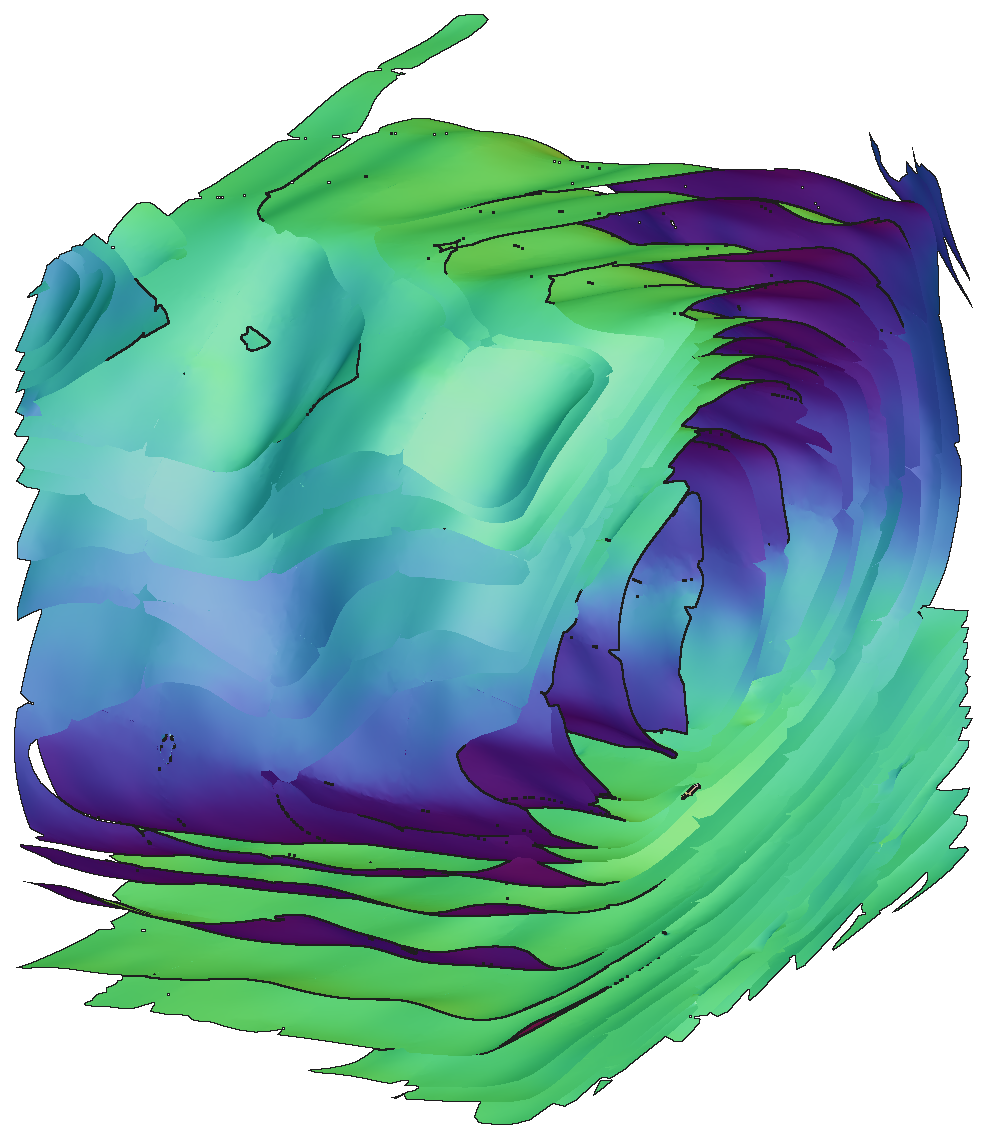
\includegraphics[width=\linewidth]{figures/teaser_geometry.png}
    \caption{Welded geometry}
    \label{fig:overview_mesh}
  \end{subfigure}
  \hfill
  \begin{subfigure}[b]{0.800\textwidth}
    \centering
    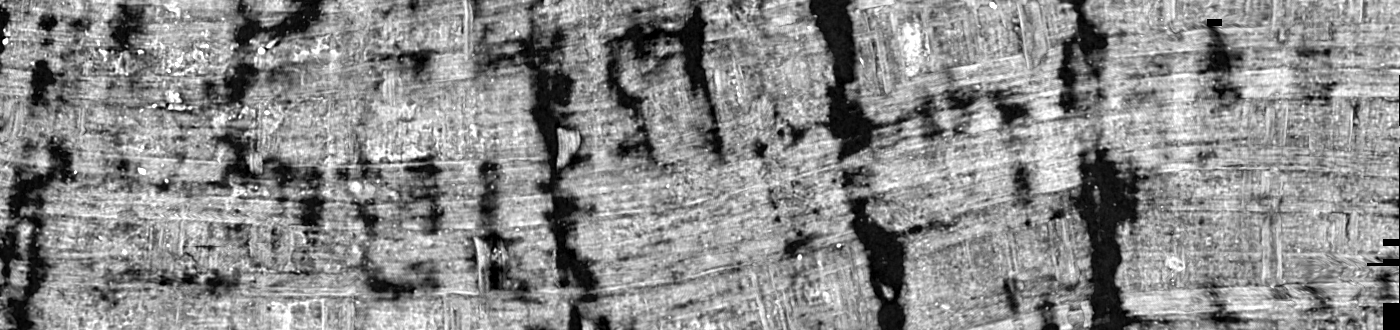
\includegraphics[width=\linewidth]{figures/teaser_ribbon.png}
    \caption{Raw CT read-back through the finished atlas --- fibre bundles run continuously across the chart seams}
    \label{fig:overview_unwrap}
  \end{subfigure}
  \caption{The current ScrollFiesta path on the $4\times5\times5$ PHerc0139 fixture, from reconstructed geometry to a readable sheet. The component-coloured weld (a) is lifted onto integer windings, which places every chart on the wrap it belongs to (Fig.~\ref{fig:tabu_winding}). Sampling raw volumetric CT data using this mesh produces the continuous fibres across seams in (b), validating that geometry, winding, and flattening are correct.}
  \Description{Two panels: a coloured concentric scroll mesh shaded by surface normal, and a wide grayscale flattened CT strip containing continuous papyrus fibres.}
  \label{fig:overview}
\end{teaserfigure}

\maketitle

% ---------------------------------------------------------------------------
% Body. One file per section under sections/; edit those, not this list.
% ---------------------------------------------------------------------------
\section{Introduction}
A vast library of papyrus scrolls was carbonized at Herculaneum during the 79 AD eruption of Mount Vesuvius. Synchrotron micro-CT preserves their internal geometry, but the ink becomes readable only after the correct papyrus surface has been found in three dimensions and {\em virtually unwrapped} to a plane. The useful computational object is therefore not a closed volume boundary. It is one consistently oriented side of an open sheet, with adjacent turns kept separate, genuine holes distinguished from meshing holes, and enough metric fidelity that fibres and writing remain continuous after flattening.

Automatic segmenters based on U-Net architectures~\cite{ronneberger2015u} provide strong voxel-level evidence, but not that object. Their predictions can be several voxels thick, contain gaps and solid blocks, or join adjacent wraps through narrow and broad {\em fusion bridges}. Standard reconstruction tools compound the mismatch: marching cubes~\cite{lorensen1998marching} and Poisson reconstruction~\cite{kazhdan2006poisson} seek a two-sided, watertight boundary. Meshing a scroll requires an algorithm that outputs a single-sided, open, and approximately developable manifold. Moreover, results that look plausible when rendered may still contain small defects; a single short edge connecting two surfaces a full turn apart can invalidate every downstream parameterization. This in turn introduces a second challenge: building a robust parameterization of the meshed scroll that corrects both for scroll damage, such as sheet delamination and physical damage to the scroll itself, as well as any errors introduced during meshing. Finally, any algorithm for scroll meshing must be parallelizable and be able to operate on small domains within the larger volumetric data, which consists of tens of thousands of cubes of voxel geometry for a single scroll.

ScrollFiesta addresses this challenge, treating meshing, topology, parameterization, and validation as one pipeline while operating on individual cubes of CT data and predictions. Given raw CT data and a matching prediction (generated by the existing nnU-Net pipelines), it constructs single-sided meshes of open sheets using a pipeline based on a compact-support moving least squares fit (MLS) combined with a guarded ball-pivoting meshing. It then separates bridged or overlapping layers, caused either by scroll damage or errors in the original prediction; fills clean boundary loops; and severs short topological handles. The resulting mesh sheets are remeshed with a domain-specific mesh level of detail algorithm, based around restricted Voronoi diagrams (RVD). Per-cube results are then joined into larger surfaces by inter-cube seam welding.

The output is then audited and parameterized according to its topology. ScrollFiesta uses a native slice-domain solve, attempting to fit a global arc-length parameterized scroll to the reconstructed mesh sheets. Simply using winding order produces invalid results, and breaks down in the presence of close together sheets; at the same time, it is also necessary to be able to parameterize the scroll even in the presence of such sheets, scroll damage, or the meshing process itself. We therefore parameterize the scroll into one long strip in UV space using a combined discrete-continuous optimization, in which scroll pieces are optimized using local winding information and then globally fit into the correct striation using a tabu search. We then use this map to identify problems such as delamination, off-sheet prediction, and seam mismatches, and repair them using a local quilting energy.

Verified local patches can be imported into VC3D's native loaders and connectors. Larger surfaces can now be exported as new, provenance-bearing {\em unverified Spiral hints}. We provide command-line tools, a public C ABI and CMake package, and a Python workflow that can stream an OME-Zarr region directly from S3.

Our technical contributions are as follows. First, we provide a local, single-sided reconstruction and topology-repair pipeline designed specifically for segmented scroll volumes. Second, we provide a CVT/RVD based level-of-detail and seam-welding scheme for scrolls with fail-closed topology gates. Third, we provide a complementary toolkit for patch and whole-scroll parameterization, based around an alternating discrete/continuous atlas unwrapping optimization in which a tabu search owns integer winding and registration owns metric placement. Fourth, we provide algorithms for principled scroll repair after unwrapping, based around quilting energy. Finally, all contributions integrate into the existing VC3D/Villa pipelines used by the Herculaneum Papyrus team.

This paper is a progress report: it describes the complete system currently implemented, including stages that work but are not yet final, and reports failures where the audits show that core topology remains unresolved.


\section{Related Work}

\paragraph{Virtual unwrapping of the Herculaneum scrolls.} Virtual unwrapping was introduced by Seales et al.~\shortcite{seales2016damage}, who recovered text from the En-Gedi scroll by segmenting its surface within a CT volume and flattening it to a plane. Applying the same idea to the far more tightly-wound Herculaneum scrolls has driven several recent automatic approaches, collected by the Vesuvius Challenge. {\em Spiral-fitting} \cite{henderson2026virtually} uses the fact that a scroll is, in its original form, a single rolled sheet, and fits an extruded spiral to the prediction by solving a variational problem; this is elegant, but degrades wherever the neural-network prediction is too noisy for any single spiral to fit. {\em Surface-tracing} approaches find small patches on the surface prediction and grow them iteratively, turning the problem into an advancing front. To the best of our knowledge, the open difficulty with this approach is how adjacent patches are merged and how the resulting topological artifacts are resolved, especially when the merge is performed after flattening the patches to two dimensions. {\em ThaumatoAnakalyptor} extracts a point cloud using blurring and Sobel edge detection, classifies the points into wraps, and reconstructs the surface by solving a winding-angle assignment problem, sharing the prediction-noise sensitivity of spiral-fitting. ScrollFiesta also grows an advancing front via ball-pivoting, but handles topology directly on the reconstructed mesh rather than in raw prediction space. In addition to avoiding the necessity of complicated front merges, this in-situ approach makes topological repair such as hole filling and bridge splitting feasible. When we do assign a winding index for the final unwrapping (Section~\ref{sec:unwrap}), we adopt the diffeomorphic-spiral idea of these methods, but apply it to the {\em repaired} mesh in a slice domain where the residual fusion bridges can be cut geometrically, rather than to the noisy prediction directly.

\paragraph{Surface reconstruction and meshing.} Surface reconstruction is a mature field, but its standard tools are a poor fit here because they are built to produce {\em two-sided, watertight} surfaces. Marching cubes~\cite{lorensen1998marching} and its descendants, such as dual contouring~\cite{ju2002dual} and the differentiable FlexiCubes~\cite{shen2023flexicubes}, extract a closed isosurface; Poisson reconstruction~\cite{kazhdan2006poisson} fits a closed indicator function and, in its distributed form~\cite{kazhdan2023distributed}, scales to large volumes. The main problem with these classical approaches is that a scroll sheet is an open, single-sided manifold: applying methods designed for closed surfaces yields two-sided envelopes that must subsequently be converted to single-sided sheets. Before designing our current approach, we investigated the possibility of meshing the Herculaneum papyri using both marching cubes and Poisson surface reconstruction as starting points. These failures motivated our current algorithm.

\paragraph{Mesh parameterization and atlas construction.} Flattening a surface to the plane is a mature area, but the classical objectives are the wrong ones here. Angle-based flattening and LSCM~\cite{sheffer2005abf++} minimize angular or conformal distortion and offer {\em no} guarantee that the resulting map is injective; on a long, high-aspect, physically damaged strip, folded and overlapping triangles are a routine outcome rather than a corner case. That is exactly the guarantee a scroll needs, so where ScrollFiesta hands a clean disk-like patch to an external flattener it uses a symmetric-Dirichlet energy~\cite{smith2015bijective}, which is locally injective by construction, and it never uses a conformal map as the final authority. A surface that will not flatten as one piece is instead cut into charts and packed into an atlas, and a body of work addresses making that packing compact and low-distortion~\cite{limper2018box}.

What all of these share is an assumption that the input surface is correct and that the remaining problem is distortion. A scroll violates that assumption twice, and both violations are structural rather than numerical. First, the correct layout is not the one that minimizes distortion. It is the one in which a chart sits exactly one circumference away from the chart one wrap inside it. That constraint is global, integer-valued, and external to the mesh: no local energy on the surface can express it, and a distortion-optimal flattening of a wrongly fused pair of wraps is still wrong. Second, the failure to avoid is not per-chart injectivity but {\em inter-chart collision} --- two different wraps occupying the same $(u,v)$ --- which a free-boundary packer has no reason to prevent, since in a conventional atlas a chart may be placed anywhere that is empty. Our slice-domain construction attacks both directly: developed length comes from measured arc length along cut strokes and is made monotone by isotonic projection, so a chart is overlap-free in $u$ by construction rather than by penalty, and the remaining inter-chart collisions are then audited exactly rather than approximated by an energy. The closest existing formulation is StrokeStrip~\cite{pagurek2021strokestrip}, which fits one common parameterization to a {\em cluster} of strokes rather than to a single connected patch; we adopt its slice-domain view and add the integer winding assignment a scroll additionally requires, solving the two as alternating discrete and continuous stages (Section~\ref{sec:unwrap}).


\section{Algorithm Overview}
\label{sec:overview}

\begin{figure*}[t]
  \centering
  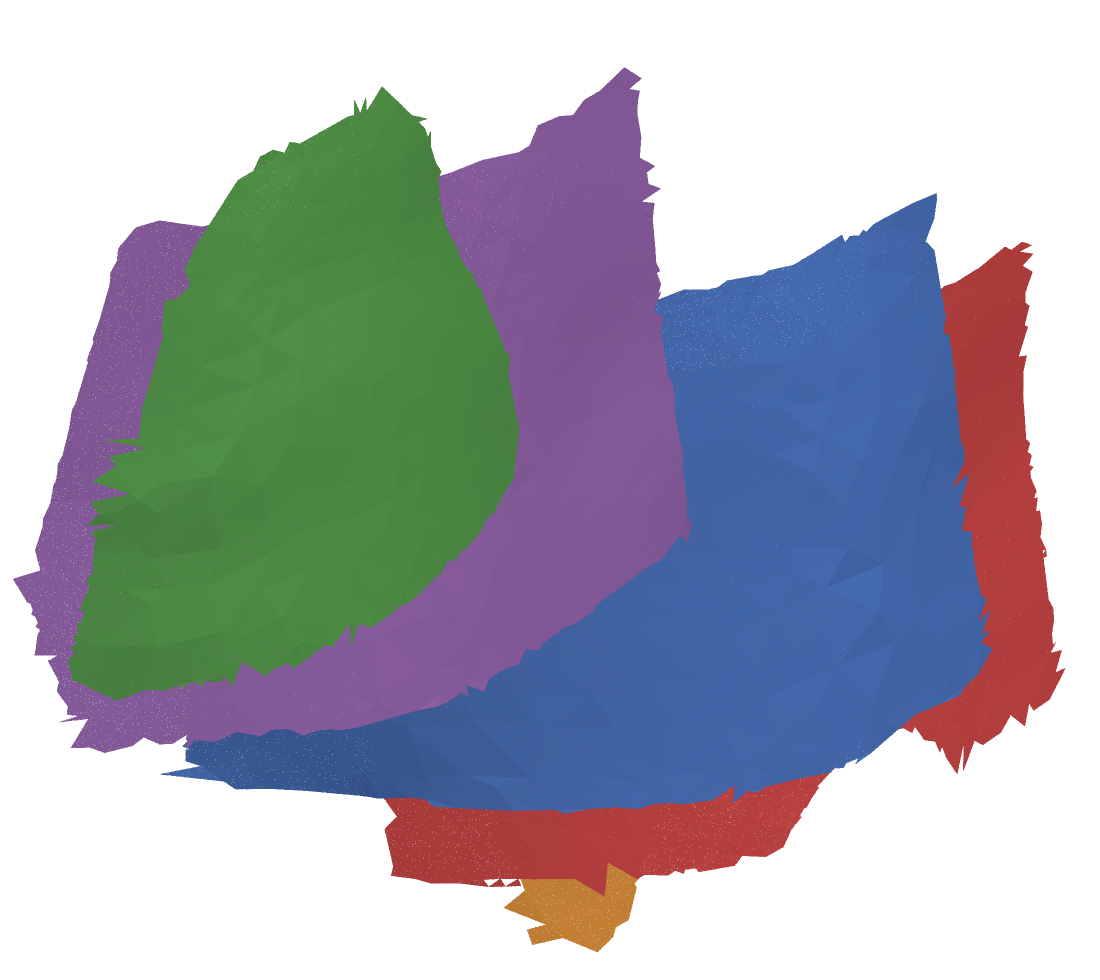
\includegraphics[height=1.13in]{figures/pipe_cube_sheets.png}\hfill
  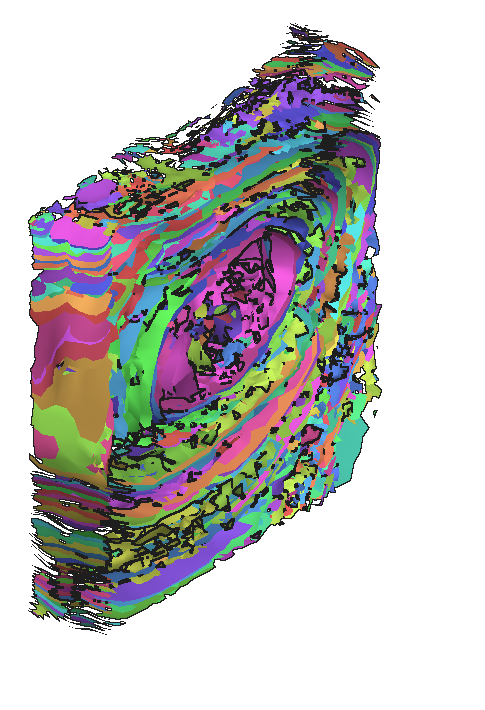
\includegraphics[height=1.13in]{figures/pipe_weld_crop.png}\hfill
  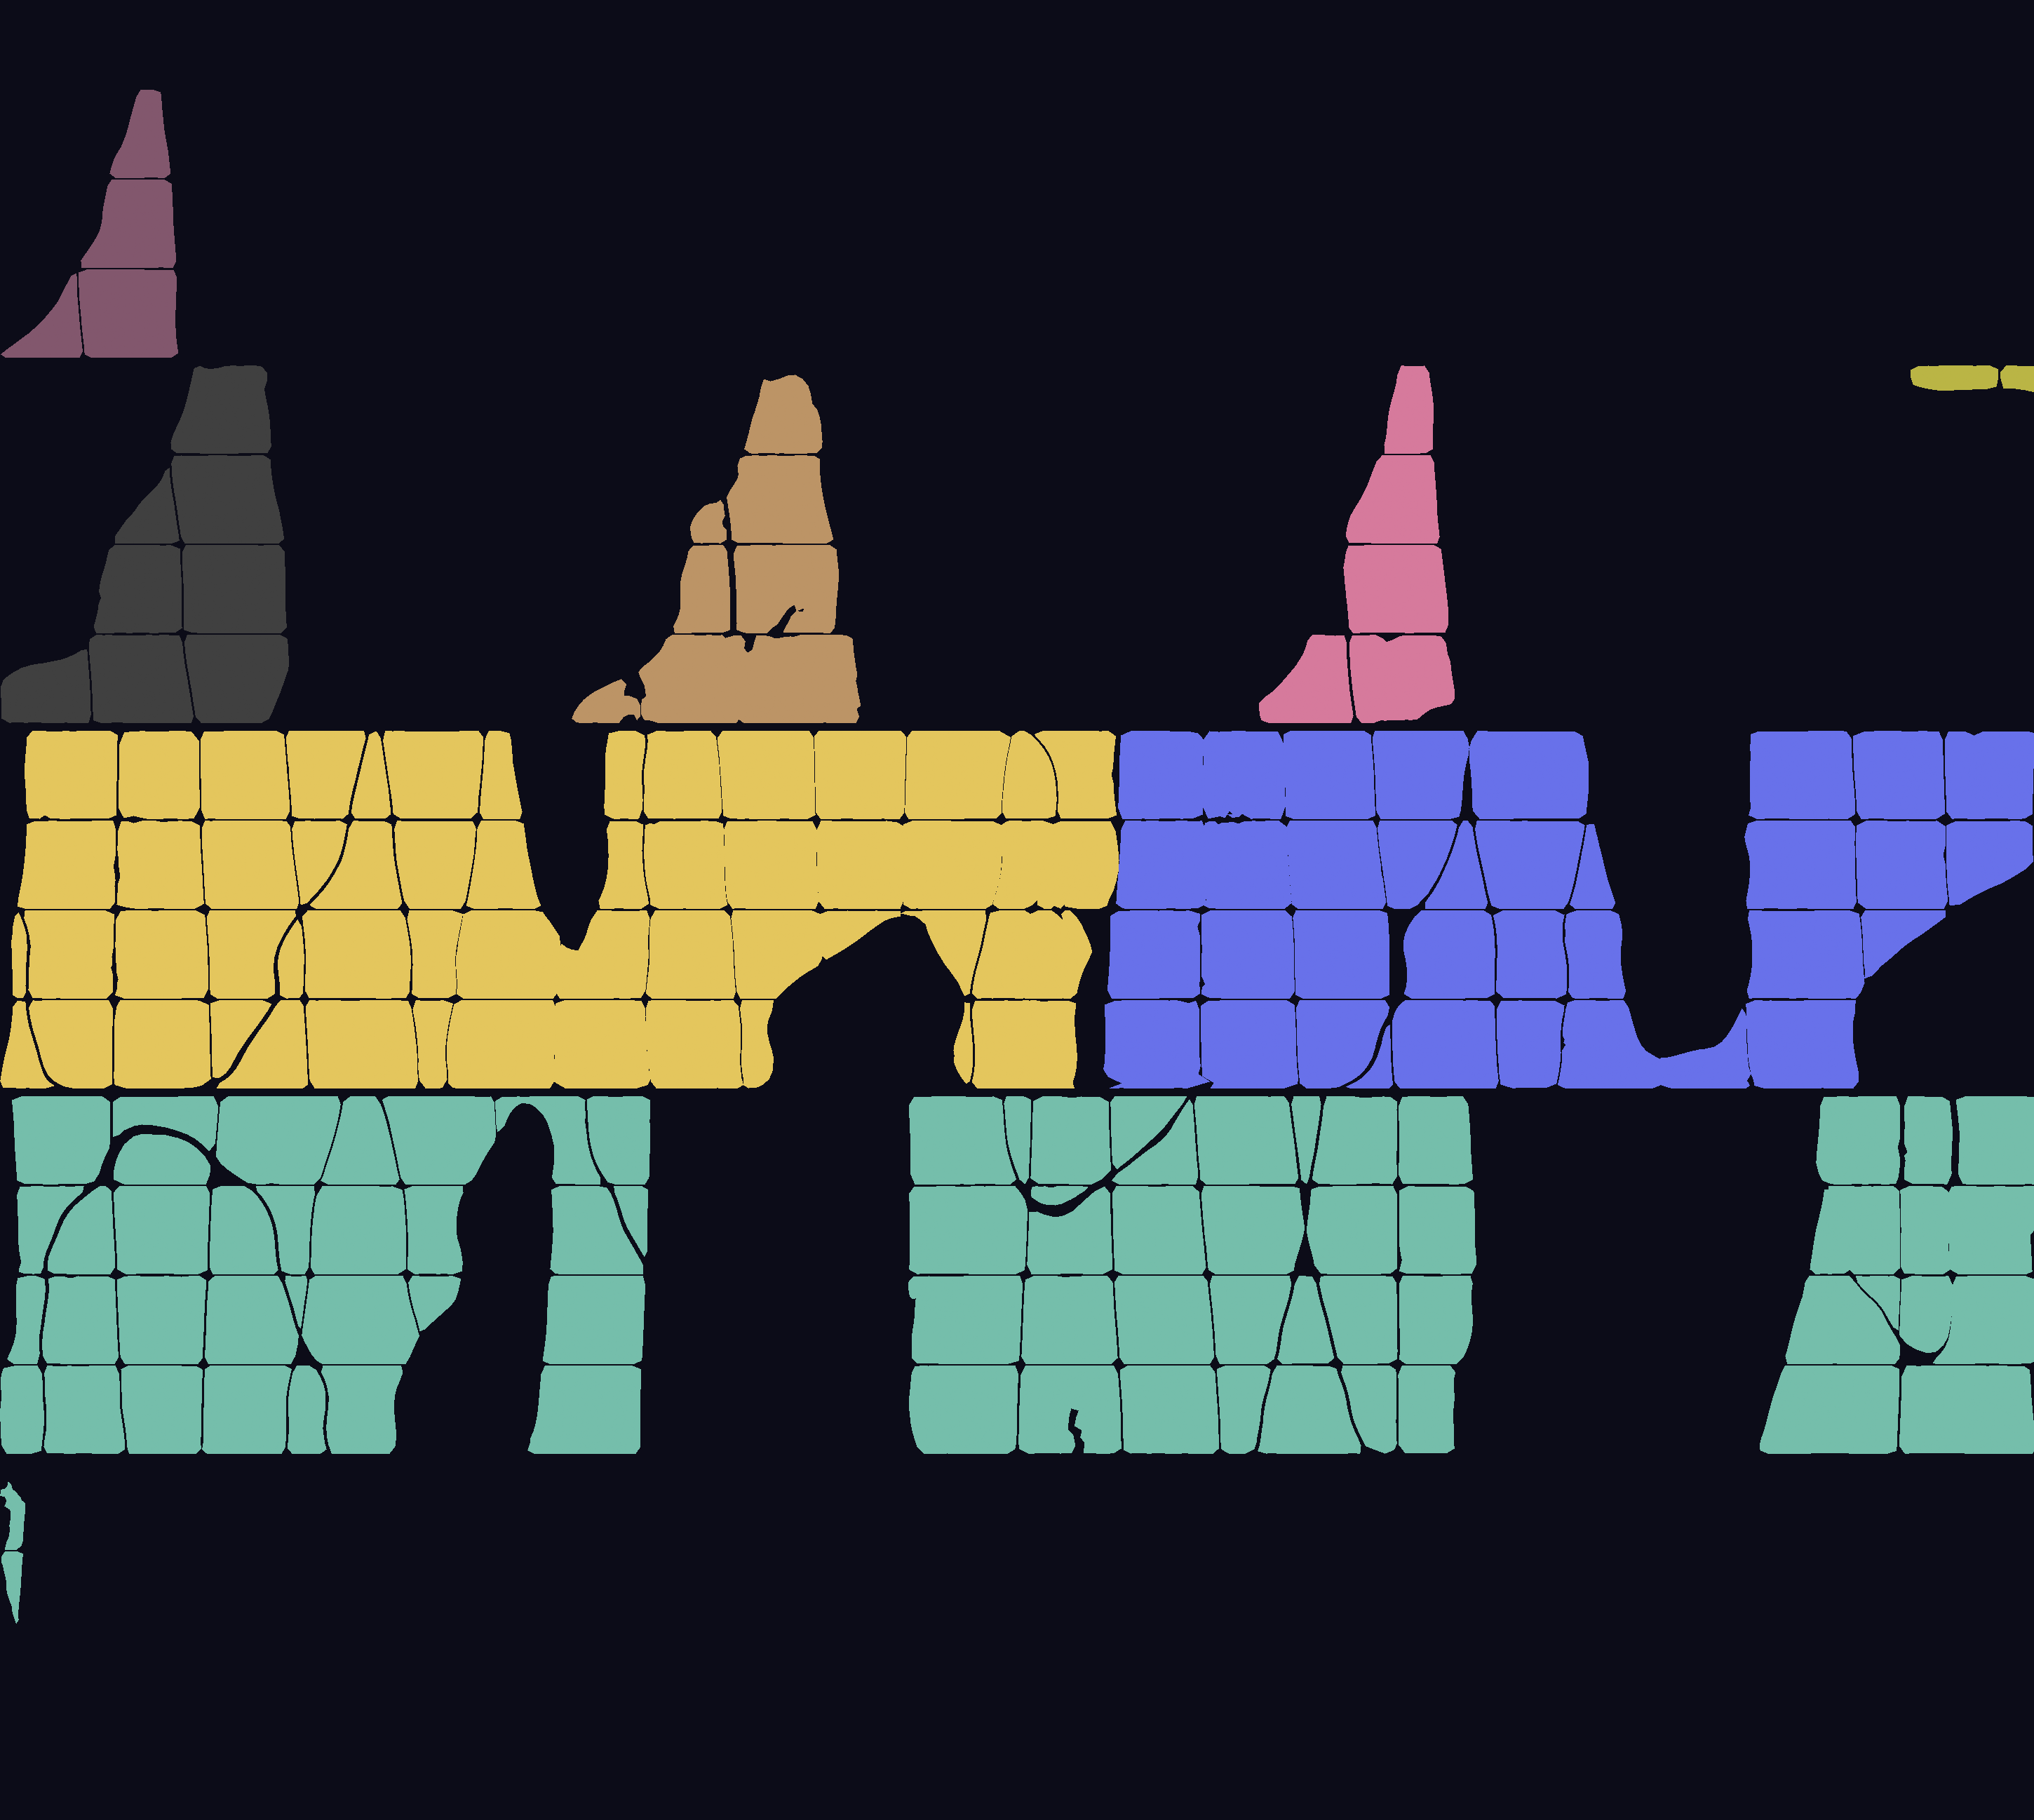
\includegraphics[height=1.13in]{figures/pipe_atlas_crop.png}\hfill
  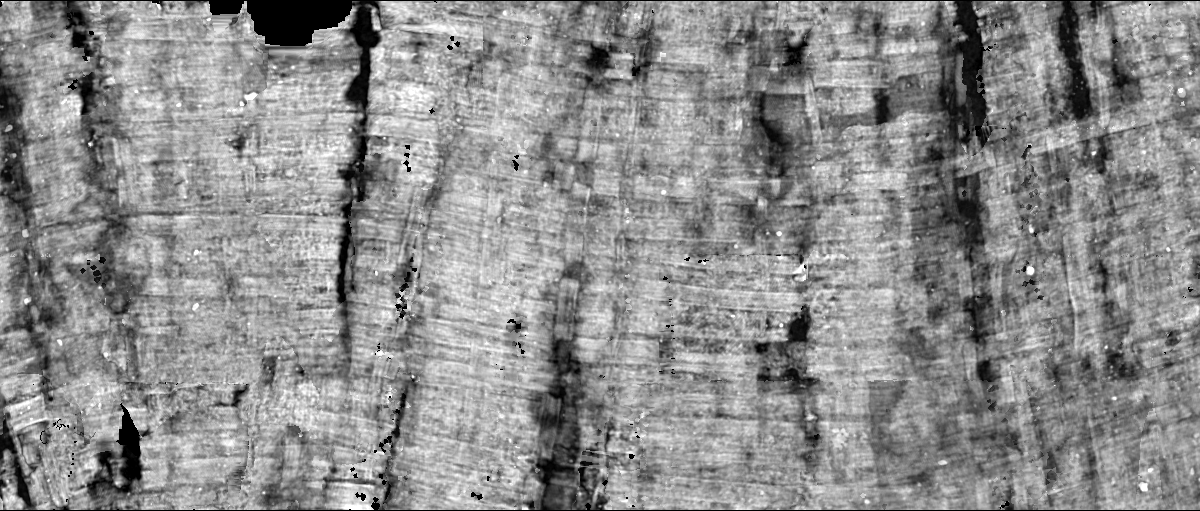
\includegraphics[height=1.13in]{figures/pipe_readback_crop.png}
  \caption{ScrollFiesta overview. Left to right: (a) each cube of thresholded U-Net evidence is collapsed to thin point sheets and meshed into separated, single-sided components (one cube's worth of the reconstructed PHerc0139 fixture shown after level of detail, component-coloured); (b) accepted cubes are CVT-remeshed and welded into a scroll block through refined seam bands; (c) the welded charts are flattened by a slice-domain metric solve, and a discrete winding lift places each welded group on its own wrap in the developed $(u,v)$ domain (detail of the lifted atlas, coloured by welded group); (d) sampling the raw CT volume through the finished map yields the readable sheet, whose continuous fibres validate geometry, winding, and flattening together.}
  \Description{Four panels: a stack of coloured papyrus sheets in one cube, a component-coloured welded scroll block with a spiral cross-section, coloured chart islands laid out in a dark flattened domain, and a grayscale CT texture strip with continuous fibres.}
  \label{fig:pipeline}
\end{figure*}

\subsection{Problem Statement}
\label{sec:problem}

ScrollFiesta takes as input a local array, or remotely stored region, of voxel evidence, normally thresholded to {\em solid} and {\em empty}, together with its world-space origin, voxel scale, cube grid, CT volume, and (for scroll-scale work) the estimated umbilicus and axis. Its output is a triangle mesh with component labels, topology and winding reports; a developed coordinate field or ribbon; sampled CT imagery; and a provenance-bearing \texttt{tifxyz} atlas. It may stop earlier with a mesh-only result, reject a bad cube, or mark downstream geometry unverified when a required gate fails.

Four requirements, established in the introduction, shape the design. First, the useful object is one consistently oriented side of an open sheet, so every stage must construct and preserve single-sided open manifolds rather than the watertight boundaries standard reconstruction produces. Second, a full scroll comprises tens of thousands of cubes, so every stage must operate on a small domain plus a fixed-radius halo and compose deterministically across cube boundaries. Third, a single wrong join --- one short edge connecting surfaces a full turn apart --- can invalidate everything downstream, so a stage that cannot certify its output must quarantine it rather than emit plausible-looking geometry. Fourth, the correct flattened layout is subject to a global, integer-valued winding constraint that no local distortion energy on the surface can express, so parameterization must jointly solve discrete and continuous unknowns rather than minimize distortion alone.

\subsection{Method Pipeline}
\label{sec:pipeline}

Mesh construction proceeds in five stages (Fig.~\ref{fig:pipeline}a,b; per-cube stages in Fig.~\ref{fig:cube_stages}). {\em Extraction} (Sec.~\ref{sec:percube}) guards each cube against degenerate predictions, collapses its voxel evidence to thin point sheets with a moving least-squares estimator, orients the sheets consistently, and meshes them with a guarded ball-pivoting front. {\em Topological repair} (Sec.~\ref{sec:cleanup}) severs thin necks and overlaps, splits pinches, fills clean interior holes, and opens non-separating handles, re-projecting and re-meshing each separated piece from its original voxel points. {\em Level of detail} (Sec.~\ref{sec:cvt}) remeshes each sheet by a restricted CVT, producing near-isotropic triangulations at a uniform budget. {\em Welding} (Sec.~\ref{sec:weld}) joins adjacent cubes through locally refined seam bands under winding gates, then recoarsens the bands by pinned CVT/RVD without disturbing the audited topology. Finally, topology and winding {\em audits} decide whether each welded sheet may be parameterized at all, and on which trust path.

Parameterization then solves for a mixture of discrete and continuous variables. The continuous variables are the developed coordinates $(u,v)$ of every vertex, where $u$ is metric developed length and $v$ is position along the scroll axis; the discrete variables are the integer winding depths of {\em charts} --- connected mesh components, in practice one cube's sheet each --- whose physically welded groupings must land exactly one circumference apart from their inner neighbours. An initial continuous field comes from a slice-domain metric solve anchored by a calibrated spiral prior (Sec.~\ref{sec:unwrap}); winding order alone is an unreliable predictor of scroll topology, so this field is only a starting point. A deterministic tabu search then owns the integers, moving charts and whole welded groups between winding depths, while a continuous re-registration owns the metric, restoring seam agreement with the chosen depths held fixed; the two alternate until no chart moves (Fig.~\ref{fig:pipeline}c). The selected map is rasterized against the CT and cleaned in the parametric domain --- overlap quilting, RAW-guided snap, seam registration, and a collision-audited ribbon fit (Sec.~\ref{sec:repair}) --- before the atlas and its CT read-back are assembled (Fig.~\ref{fig:pipeline}d) and handed off on an explicitly verified or unverified path (Sec.~\ref{sec:integration}).

Sections~\ref{sec:percube}--\ref{sec:repair} describe each stage in detail. Throughout, we state each energy in the form the implementation optimizes; Appendix~\ref{app:terms} collects the precise definition of every term, the default constants, and the complete tabu-search procedure, so that each stage can be reproduced without reading the source.

\section{Per-Cube Mesh Extraction}
\label{sec:percube}

\begin{figure*}[t]
  \centering
  \begin{subfigure}[b]{0.24\linewidth}
    \centering
    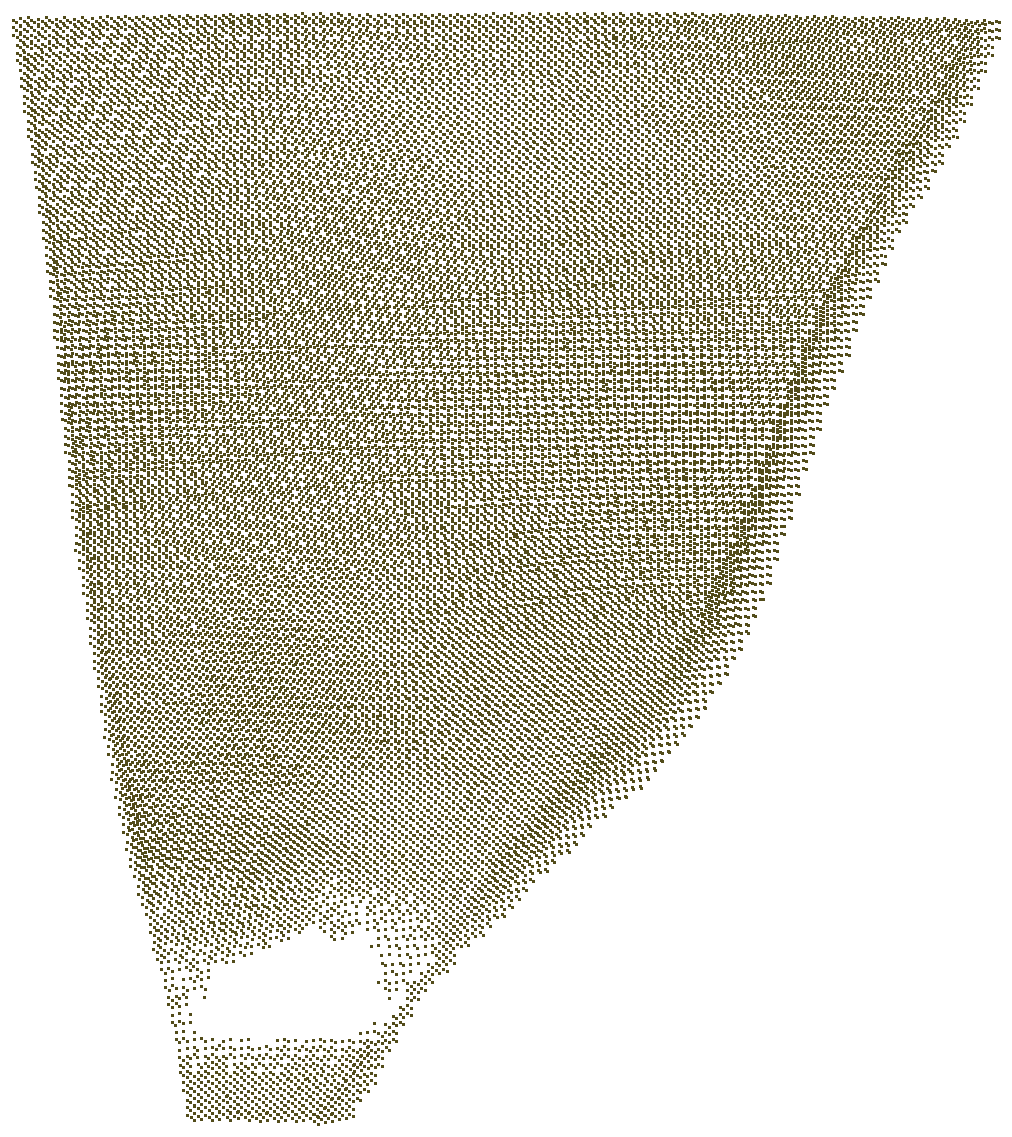
\includegraphics[width=\linewidth]{figures/overview00_crop.png}
    \caption{MLS-collapsed points}
  \end{subfigure}
  \hfill
  \begin{subfigure}[b]{0.24\linewidth}
    \centering
    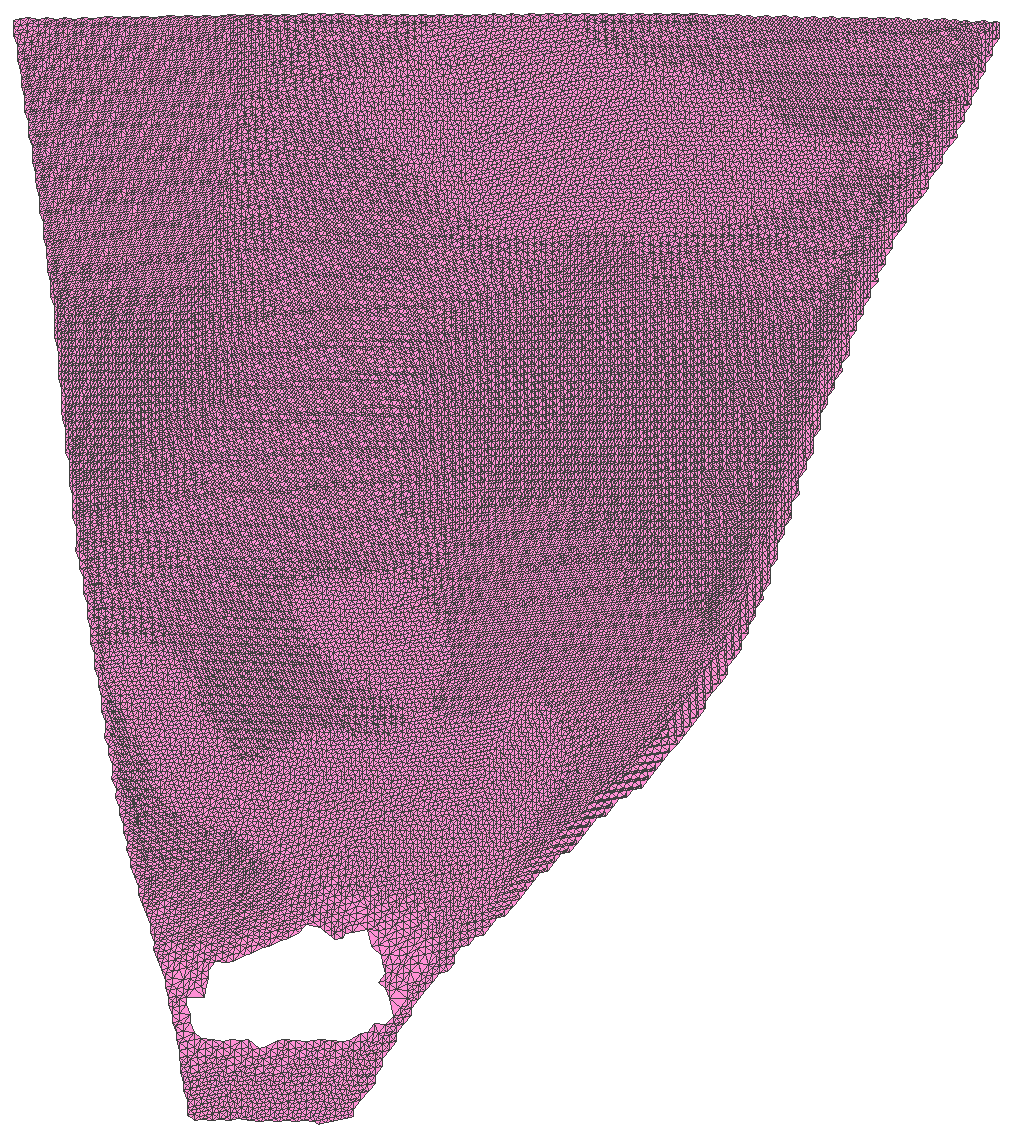
\includegraphics[width=\linewidth]{figures/overview01_crop.png}
    \caption{Guarded ball pivoting}
  \end{subfigure}
  \hfill
  \begin{subfigure}[b]{0.24\linewidth}
    \centering
    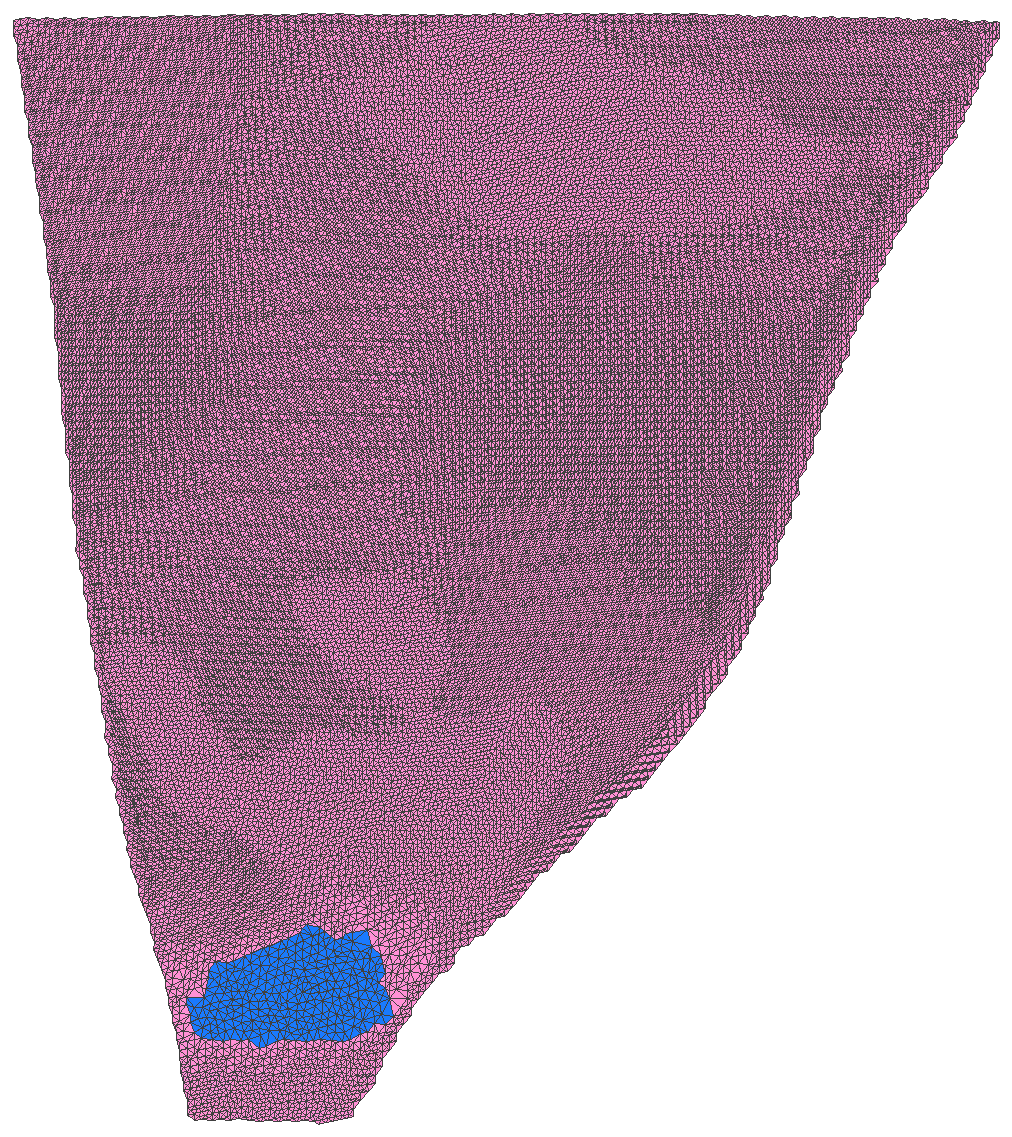
\includegraphics[width=\linewidth]{figures/overview02_crop.png}
    \caption{Interior loops filled (blue)}
  \end{subfigure}
  \hfill
  \begin{subfigure}[b]{0.24\linewidth}
    \centering
    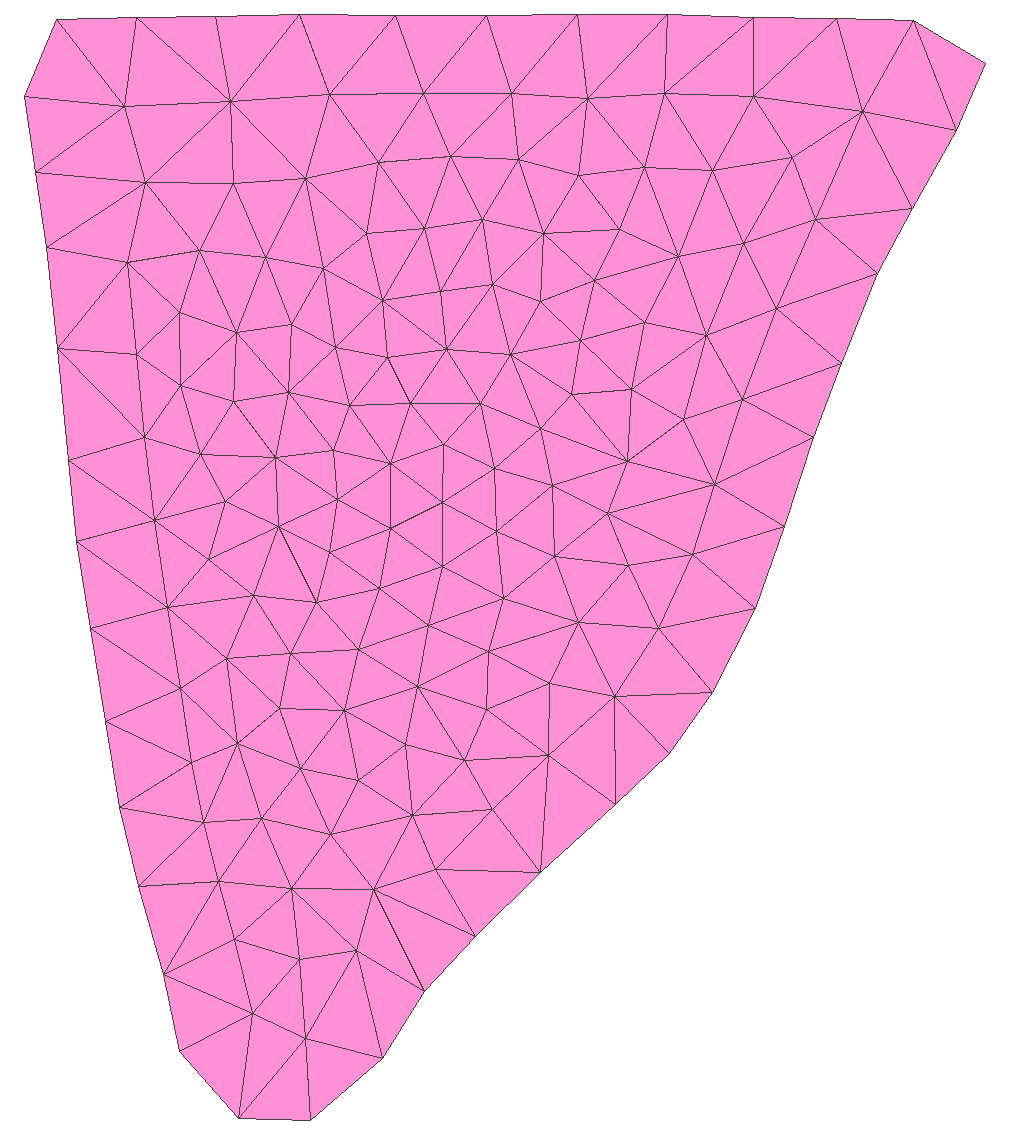
\includegraphics[width=\linewidth]{figures/overview03_crop.png}
    \caption{CVT/RVD remesh}
  \end{subfigure}
  \caption{The per-cube extraction stages on one PHerc0139 sheet. (a) Voxel-centre points after the iterated MLS projection has collapsed the several-voxel-thick prediction to a single sheet. (b) The consistently oriented, guard-gated ball-pivoting reconstruction; the remaining perforations are prediction gaps. (c) Clean interior loops are closed (filled regions shown in blue) while the genuine sheet boundary is left open. (d) The level-of-detail stage on the same sheet: the CVT/RVD remeshing of Section~\ref{sec:cvt} relocates samples into a near-isotropic blue-noise distribution.}
  \Description{Four panels showing the same roughly triangular papyrus sheet as a dotted point cloud, a dense pink triangle mesh with holes, the same mesh with blue filled patches, and a coarse triangulated version.}
  \label{fig:cube_stages}
\end{figure*}

Before meshing a cube we apply a lightweight input guard. A U-Net occasionally emits a degenerate prediction in which a region is filled as a solid block rather than a thin sheet; ball-pivoting cannot roll across a solid three-dimensional point fill, and meshing such a cube yields only fragmented debris. We detect these cubes by morphological erosion-survival: a small 3D erosion dissolves a genuine thin sheet entirely while a solid slab retains a large interior fraction. We additionally require that the surviving foreground form a solid filled rectangle across many consecutive slices, so that dense but legitimate wrap regions are never rejected. A cube that fails this guard is skipped and contributes nothing to the output rather than junk geometry.

We initialize our point cloud by extracting one point at the centre of each solid voxel of the input cube. Where the prediction is more than one voxel thick this yields a slab of points several voxels deep, so we first collapse and denoise it into a single clean sheet using an iterated moving least-squares (MLS) projection~\cite{levin2003mesh}: each point is moved along its local surface normal, estimated from a Wendland-weighted neighbourhood~\cite{wendland1995piecewise}, onto the local least-squares plane. Only the through-thickness component of this motion is non-zero, so the slab is thinned to a single sheet without the in-plane contraction we observed when we initially tried the closely-related locally optimal projection~\cite{lipman2007parameterization}. The projection itself is a standard tool; our observation is that choosing a projection method whose kernel has compact support makes the per-cube result consistent across cube boundaries, and that this boundary-consistency is precisely what makes our divide-and-conquer scroll meshing possible. Concretely, adjacent cubes are processed with an overlapping halo of shared input voxels, and because each projected position depends only on neighbours within a fixed radius, points in the shared region land in the same place in both cubes; the two cubes therefore present matching geometry to the welder. Finally, we trim the cloud so that the open mesh boundary falls inside the cube face, and weld points lying within 0.25 voxels of one another.

We then assign the point cloud a globally consistent normal orientation using the method of Hoppe et al. \shortcite{hoppe1992surface}, to ensure that all papyrus surfaces are consistently oriented as our algorithm requires. 

Meshing the point cloud requires an algorithm that is local (in order to join cubes together after processing); fast; and that is not designed to output a closed, watertight surface. We therefore use the ball-pivoting algorithm \cite{bernardini1999ball} (BPA), which we summarize as follows: three points form a triangle if a ball of a user specified radius $\rho$ touches them without containing any other point. Starting with a seed triangle, the ball pivots around each edge until it touches another point, forming a triangle. The process continues until all reachable edges have been tried, and then starts from another seed triangle until all points have been considered. We found that this simple approach satisfies our main criteria, at the cost of some small topological artifacts which are easily resolved (see below): it can be used to weld neighbouring cube surfaces into the complete scroll by setting the cube boundaries to the advancing front at the algorithm start, and it is very well-behaved on open surfaces. Our implementation of BPA includes several guards that keep the advancing front on a single sheet. A dihedral fold-back guard prevents the front from folding back over itself. A face-coherence guard rejects any candidate triangle whose normal turns too sharply away from the triangle that owns the pivot edge; without it, the ball tends to roll down onto an adjacent wrap instead of across a thin gap in its own sheet, stitching the two layers together. An anti-parallel guard similarly refuses to add a triangle that would bridge two oppositely-oriented surfaces lying close together, as occurs where neighbouring wraps nearly touch. A {\em wall guard} rejects candidates that are simultaneously steep against the local MLS normal and long: a fusion bridge stands nearly perpendicular to the sheet it fuses and must reach across the inter-wrap gap, whereas a genuine surface triangle is parallel to its vertex normals, so the conjunction fires only on through-thickness bridges and spares sharp folds. Finally, because a front can accumulate error gradually --- every individual pivot innocent while the front slowly climbs a through-thickness wall and gains whole turns --- each seed's growth carries a branch-cut-free integrated winding phase about the scroll axis, and a pivot whose accumulated phase leaves a tolerance band is refused; the surface beyond it is re-seeded as a distinct component. Guard thresholds appear in Appendix~\ref{app:terms}.

\paragraph{Quality-gated extraction.}
A smaller pivot radius can sometimes avoid a local fusion, but it can also discard surface coverage and explode the number of open boundary edges. We therefore do not tune $\rho$ by appearance. The adaptive controller begins at the normal radius and only tries smaller radii after a winding failure. A candidate is accepted only when it contains no abrupt full-turn edges or broad branch-local fusions, retains at least 95\% of the baseline point coverage, and introduces no more than 1.25 times the baseline boundary edges. If no candidate passes, the component is quarantined for cutting or an unverified downstream path. This makes the extraction decision part of the topology audit rather than an undocumented per-dataset parameter choice.

\subsection{Topological Cleanup}
\label{sec:cleanup}

A single voxel connected-component can hold several {\em disconnected} surface sheets that were projected and meshed together, because the moving least-squares projection operates on all of a component's points at once and nearby sheets pull on one another. Before anything else, we separate each meshed component into its connected pieces and re-project and re-mesh each one in isolation, this time from its {\em original} voxel-center points rather than from the already-projected vertices, so that the projection kernel sees only same-sheet neighbours and each sheet lands cleanly on its own surface. Re-projecting from the original points proves to be a reusable primitive, which we also apply after every split below to clean the ragged boundary a cut otherwise leaves behind.

At this stage, we may have multiple components erroneously attached in the same cube. This can be due either to proximity during the BPA algorithm, or more commonly due to errors in the input. As we now have meshes, we can detect these connections by finding every connected mesh component in the cube, and casting rays from each triangle centroid along its normal in both directions to determine if we should split the input geometry.

We categorize splits into two cases. First, we consider the case where one small bridge connects two levels of geometry; this is commonly caused by scroll NN prediction artifacts (Fig.~\ref{fig:bridgesplit}). We formulate finding these splits as a min-cut problem, and we solve it using the standard Edmonds-Karp algorithm. For more complex overlapping geometries, we use a lifted multicut solver \cite{keuper2015efficient} to solve an overlap reduction problem based on the formulation from Limper et al. \cite{limper2018box}. After splitting, each resulting piece is re-projected and re-meshed from its parent's original voxel points as described above, so that the new sheet boundaries come out clean rather than carrying the jagged trace of the cut.

\begin{figure*}[t]
  \centering
  \begin{subfigure}[b]{0.245\linewidth}
    \centering
    
\includegraphics[width=\linewidth]{figures/neck_before00.png}
    \caption{Fused pair, before}
    \label{fig:bridgesplit_before}
  \end{subfigure}
  \hfill
  \begin{subfigure}[b]{0.245\linewidth}
    \centering
    
\includegraphics[width=\linewidth]{figures/neck_after01.png}
    \caption{Severed at the neck}
    \label{fig:bridgesplit_after}
  \end{subfigure}
  \hfill
  \begin{subfigure}[b]{0.245\linewidth}
    \centering
    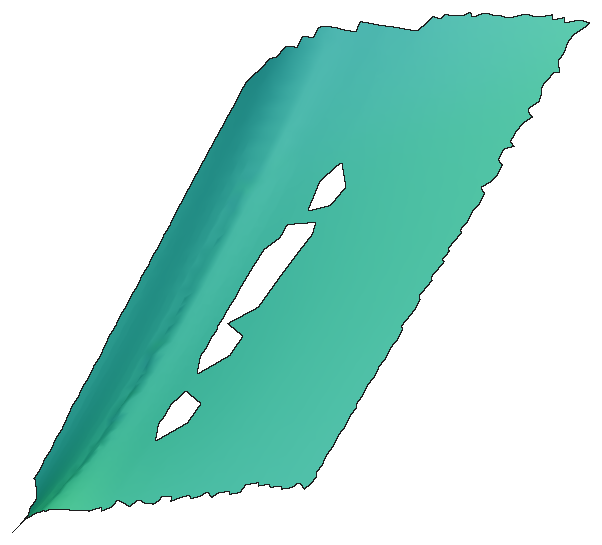
\includegraphics[width=\linewidth]{figures/holefill_before.png}
    \caption{Perforated sheet, before}
    \label{fig:holefill_before}
  \end{subfigure}
  \hfill
  \begin{subfigure}[b]{0.245\linewidth}
    \centering
    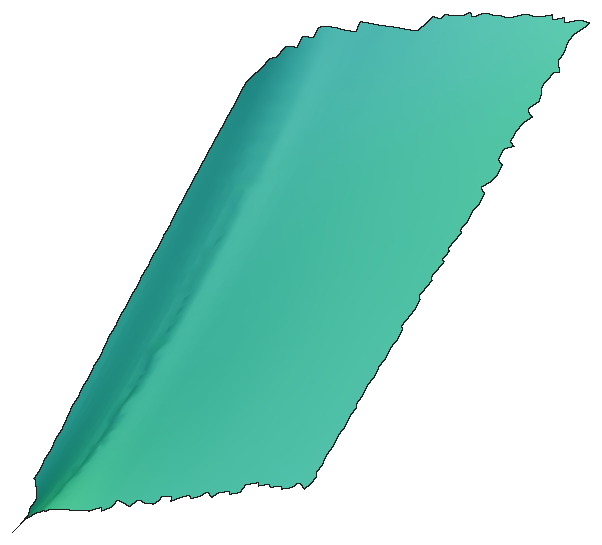
\includegraphics[width=\linewidth]{figures/holefill_after.png}
    \caption{Interior loops closed}
    \label{fig:holefill_after}
  \end{subfigure}
  \caption{The two mesh-space repairs that must happen before any parameterization is attempted, on real PHerc0139 cubes. (a,b) The U-Net has fused two sheets through a thin neck of bridge material; the bridge is detected and severed by min-cut, recovering two distinct sheets --- a fusion left in place would weld two wraps into one and make the winding topology unrecoverable. (c,d) Holes left by the ball-pivoting front and by gaps in the prediction are closed: exact three-edge loops directly, larger clean interior loops by constrained Delaunay with Liepa-style refinement~\cite{liepa2003filling}. Self-intersecting, non-manifold, or clearly exterior loops are rejected rather than force-filled, so a genuine sheet boundary is never sealed shut.}
  \Description{Four small panels: two mesh sheets joined by a thin bridge and then separated at it, followed by a perforated triangle mesh and the same mesh with its interior holes closed.}
  \label{fig:bridgesplit}
\end{figure*}

After each separation we split pinched vertex fans until every stage component is vertex-manifold. If holes are detected inside a component, we patch them at this stage (Fig.~\ref{fig:bridgesplit}c,d). Exact three-edge loops are closed directly. Other clean interior loops are projected to a local plane, triangulated by constrained Delaunay, and lifted back with Liepa-style refinement~\cite{liepa2003filling}; self-intersecting, non-manifold, or clearly exterior loops are rejected rather than force-filled.

Ball-pivoting can also fuse a sheet to itself without disconnecting it: where the advancing front rolls across a thin gap, it can close a loop that raises the sheet's genus into a small handle. Such handles are {\em non-separating}, so the cut-based splitters above, which sever {\em separating} necks, cannot remove them. After hole filling, we apply a tree--cotree decomposition and open every non-separating loop shorter than a fixed length bound by manifold-preserving vertex duplication. This reduces accidental local genus while leaving the long, scroll-scale cycles that represent genuine structure untouched.

\subsection{CVT/RVD Remeshing}
\label{sec:cvt}

Previous versions of ScrollFiesta used QEM for downsampling the ball-pivoting stage output. In practice, we found that this created numerous small sliver triangles and an uneven distribution of samples. We therefore perform level of detail using a centroidal Voronoi tessellation restricted to the reconstructed surface. We seed interior sites by area and boundary sites along every retained loop, then iterate the variational update of CWF~\cite{xu2024cwf}: each interior site solves a small fixed-cell system combining the ordinary centroidal (CVT) term with a normal-anisotropy term that pulls samples onto creases and thin features, with the CVT weight decaying across iterations (Appendix~\ref{app:terms}). Each updated site is projected back to the source surface, and the output triangles are the restricted-Delaunay dual of the restricted Voronoi diagram (RVD). Uniform density is used per cube at present. Unlike collapse-only QSlim/QEM, this operation relocates samples into a near-isotropic distribution, reduces slivers, and does not preserve a poor advancing-front tessellation merely because it arrived first.

Any component above the current size cap, an empty or invalid dual, or a result that fails the manifold checks falls back to the repaired QEM path; QEM can also be selected explicitly. The fallback rejects edge collapses or maintenance flips that would create an existing edge or reverse winding. Once remeshed, components with negligible area are removed as debris, and halo output is cut at the owned cube planes so that every geometric region has a single owner at assembly time.
\section{Global Cube Welding}
\label{sec:weld}

We first place every accepted cube mesh in volume coordinates and concatenate it under the ownership established by halo trimming. The uniformly coarse CVT interiors are desirable for scale, but their triangles are too large for the weld's ball of radius at most three voxels to initialize reliably. We therefore detect every internal cube plane and refine only a narrow seam band to approximately 3.5-voxel triangles (Fig.~\ref{fig:weld_bands}). Boundary half-edges in that band seed the same BPA used per cube, and four sub-processes then connect matching fronts while refusing invalid joins. A sliver cull first removes near-degenerate boundary triangles that would prime the bridge ball off a needle. The bridge front itself escalates its radius adaptively from the local boundary spacing, capped so that twice the maximum radius stays below the measured $\sim$7-voxel inter-wrap clearance --- welding two wraps together is therefore geometrically impossible for the bridge, not merely penalized. Every candidate bridge face must also pass a {\em winding gate}: its winding-phase gap $w = r/p - \theta/2\pi$ between front and candidate must stay within a soft tolerance (0.35 turns, with a 0.40-turn hard cap that separates legitimate grazing-seam closures from cross-layer and next-wrap stitches), which also keeps recto from welding to verso. Finally, a sheet-correspondence pass recovers legitimate same-sheet closures the conservative gate refused: it confirms a mutual-best 1:1 sheet pairing across each seam from bridge votes and boundary overlap, then re-welds only that confirmed pair on a point cloud restricted to those two sheets.

After each weld is complete, the temporary fine band is recoarsened and optimized with a {\em pinned-boundary} CVT/RVD pass. Boundary positions are held bit-exact while interior sites solve the same centroidal and normal-anisotropy objective as Section~\ref{sec:cvt}. A proposed band patch is accepted only if every pin is represented, the complete boundary-edge set is unchanged, all edges remain manifold, and both component count and Euler characteristic equal their pre-remesh values. Tiled passes with an offset allow long seams to be processed at bounded memory. If any invariant fails, that tile retains the pre-CVT weld.

We note that orientation consistency alone is insufficient to guarantee a valid scroll: a perfectly manifold bridge may still connect turns that are far apart in scroll phase. The global audit therefore measures abrupt full-turn edges and also computes a branch-local phase span, which detects broad fusions assembled from individually plausible edges. A phase sever can remove faces crossing those discontinuities, but its output remains unverified until every resulting component also satisfies the broad-span test. 

\begin{figure}[t]
  \centering
  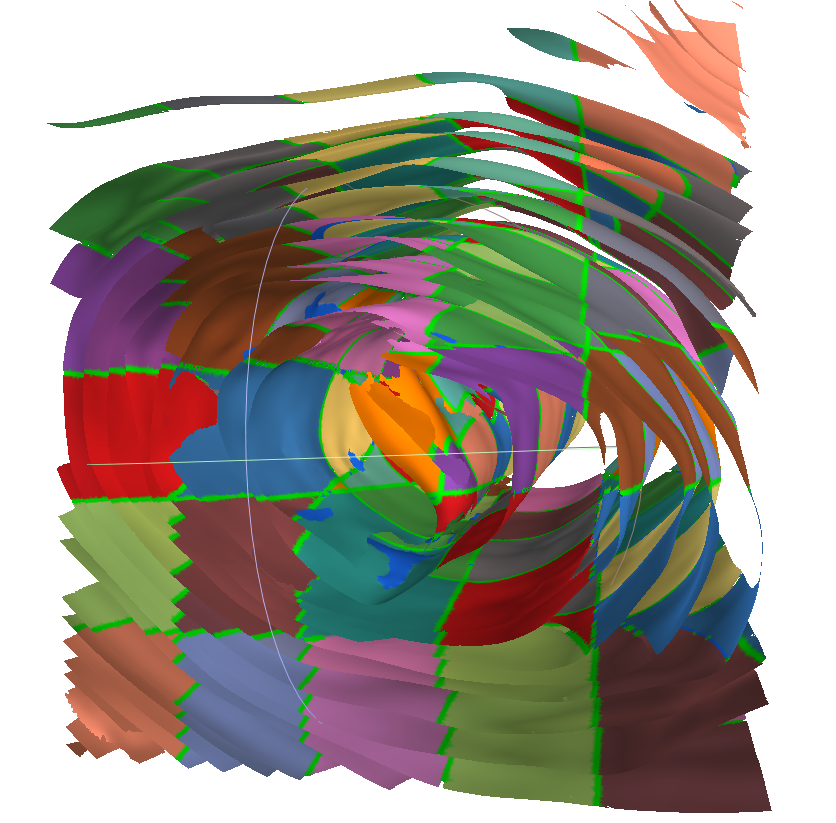
\includegraphics[width=\linewidth]{figures/welded_cube_4x5x5.png}
  \caption{The welded $4\times5\times5$ block with each cube's sheet coloured independently and the refined seam bands drawn in green. The weld bridges the $\sim$1-voxel trim gap between adjacent cubes only inside these bands; the winding gate and the capped bridge radius decide which fronts may join, so a sheet continues across a seam exactly when the two cubes agree it is the same wrap.}
  \Description{A rendered stack of curved papyrus sheets divided into cube-sized coloured tiles, with thin green bands marking the welded cube boundaries.}
  \label{fig:weld_bands}
\end{figure}

This weld is designed to compose hierarchically: a group of placed cubes or previously welded blocks enters the same seam-band procedure. The current complete validation is a flat $4\times5\times5$ block; the long $4\times21\times21$ experiment is decomposed into axial strips at the atlas level while the fully hierarchical geometry weld remains active work. In particular, our unwrapping and parameterization stage does not require the full weld, but uses it as a sub-engine to determine whether two sheets next to each other in UV space are in fact valid neighbours in the scroll itself.

\section{Unwrapping the Welded Sheet}
\label{sec:unwrap}

Virtual unwrapping requires a planar coordinate and a 3D point for every valid texel. We use two parameterization paths because a clean local patch and a long multi-turn shell have different topology and different evidence. Both paths end in the same \texttt{tifxyz} representation, CT read-back, and provenance checks.

\subsection{Verified Local Patches}

A disk-like component with a clean boundary can use a conventional free-boundary map. ScrollFiesta first creates a working ribbon so that overlaps and RAW-guided corrections can be inspected in a regular domain, applies the quilting and snap operations of Section~\ref{sec:repair}, and then hands the corrected 3D patch to Villa's maintained \texttt{flatboi} flattener, run under a symmetric-Dirichlet energy~\cite{smith2015bijective}. We use that energy rather than a conformal or angle-based map because it is locally injective by construction: on a long, damaged, high-aspect patch the failure that matters is a folded or overlapping chart, not a few degrees of angle distortion. The result is accepted as a verified patch only after its coordinates, valid-cell and quad masks, and surface-index overlaps load through Villa's official \texttt{tifxyz} and connector code. This delegation is deliberate: our optional in-house relaxation remains useful experimentally, but is not the final authority for a verified disk.

\subsection{Native Wrapped-Sheet Parameterization}

An off-the-shelf disk flattener is a poor fit for a long spiral of many turns. The desired horizontal coordinate is metric developed length, while the absolute wrap of an independently processed cube is known only up to an integer. Treating these as one continuous problem caused two distinct failures: a locally smooth field advanced only 10.3\% of the circumference owed per radial turn, and a continuous registration could not choose among whole-turn chart gauges. The current pipeline therefore separates local metric flattening from global integer winding. It combines a StrokeStrip-style slice domain~\cite{pagurek2021strokestrip}, diffeomorphic-spiral geometry~\cite{henderson2026virtually}, and a tabu search over chart depths~\cite{glover1989tabu}.

\paragraph{Setup and exact slice strokes.} The unwrapper operates on one connected sheet at a time. Small non-separating handles are first cut by the bounded-memory tree--cotree procedure of Section~\ref{sec:cleanup}. Planes perpendicular to the measured scroll axis intersect the triangles in polylines that are chained by mesh-edge identity, avoiding tolerance-based endpoint joins. Let $s\in\{-1,1\}$ be the winding sense, $p$ the pitch in voxels per turn, $r$ the radius from the umbilicus, and $\theta$ the wrapped angle; $\operatorname{unwrap}$ maps an angle difference to its principal value in $(-\pi,\pi]$. For consecutive samples $i,j$, the branch-cut-free geometric winding increment is
\begin{equation*}
  \delta w_{ij}=s\frac{r_j-r_i}{p}-\frac{\operatorname{unwrap}(\theta_j-\theta_i)}{2\pi},
\end{equation*}
which is zero on a perfect spiral ramp and accumulates $\pm1$ per wrap crossed by a fusion.
A stroke is cut when its accumulated $\delta w$ crosses a half-turn from its current anchor. This catches the actual failure found in the $4\times5\times5$ weld: plane-slice chains can snake through locally short CVT fusion edges and traverse several wraps without one dramatic radius jump. Cross-slice and within-slice continuation candidates are then admitted only when their geometric winding, distance, and tangent evidence agree; a cut endpoint cannot be joined back across the same wrap crossing.

\paragraph{Metric LS--PAVA solve.} Each surviving stroke contributes unit-speed arc-length rows, while accepted cross-sections and continuations contribute alignment rows. A radius-anchored geometric coordinate
\begin{equation*}
  \varphi_{\mathrm{geo}}=\theta+2\pi\operatorname{round}\!\left(s\frac{r}{p}-\frac{\theta}{2\pi}\right)
\end{equation*}
sets an absolute gauge only on strokes whose geometric coordinate agrees with their measured arc length; untrusted strokes do not receive a strong prior. The solve is LS--PAVA: an anchors-only reduced least-squares system over the stroke parameters --- the arc-length and alignment rows above, with a small Tikhonov term on near-null directions --- alternated with a per-stroke pool-adjacent-violators projection~\cite{barlow1972statistical}, the exact linear-time Euclidean projection onto the monotone cone, applied after each robust reweighting round. Enforcing monotonicity by projection rather than by inequality constraints inside the solver keeps every round a plain sparse least-squares problem; Section~\ref{sec:results} measures an active-set QP formulation of the same monotone system for comparison. The axial coordinate $v$ remains position along the scroll axis.

\paragraph{Direct transfer and shape preservation.} Slice coordinates are transferred to mesh vertices only when the nearest supported sample passes the distance gate. Median neighbour fills remain available to diagnose holes and to propagate later fills, but they are not marked as direct support; a face touching any non-direct vertex is excluded from the atlas. This prevents repeated fill values from creating zero-area UV plateaus. The global field application is likewise rigid at chart scale: a robust support-to-chart registration chooses one additive $u$ shift per connected raw chart. It cannot change a local edge difference, flip a triangle, or concentrate hundreds of units of mismatch in one face as the earlier dense extension did.

\paragraph{Integer winding as tabu search.} The registered field preserves local shape but leaves each of its $C$ charts an unknown integer depth $k_c\in[-K,K]$ ($K{=}4$), where a {\em chart} is one connected mesh component (in practice one cube's sheet) and a {\em welded group} is a connected component of the authentic-neighbour graph: two charts are authentic neighbours when they lie within the weld's own bridging distance with agreeing contact normals, i.e.\ when the geometric seam weld would join them into one surface. A depth move shifts a chart in $u$ by the measured field's own {\em one-wind ladder} at its local radius --- the median signed $\Delta u$ between radially adjacent same-$u$ chart pairs one wrap apart. Measuring the ladder from the field is essential because its sign on the real field is opposite the analytic spiral convention. The canonical discrete energy is
\begin{equation*}
 E(k)=\lambda_o N_{\mathrm{ov}}(k)
   +\lambda_n\!\sum_{(a,b)\in\mathcal E}w_{ab}
      \left|(k_a-k_b)-t_{ab}\right|
   +\lambda_r\!\sum_c H(k_c-\widehat{k}_c).
\end{equation*}
$N_{\mathrm{ov}}$ counts exact overlapping UV triangle pairs between charts that are not authentic neighbours ($\lambda_o{=}1$ per pair). $\mathcal E$ contains the trusted topology relations: weld edges, whose weight $w_{ab}$ is their physical contact count and whose target $t_{ab}$ is the weld's own gauge evidence --- the contact's $u$ difference divided by the local circumference, rounded to the nearest integer and trusted only when the residual is below $0.25$ turns --- and same-wind {\em lateral} relations with $t_{ab}=0$, which couple charts at the same radius in adjacent cubes that a hole or trimmed seam separates (without them the search tears such pairs apart for free). Edges inside a {\em happy family} --- a welded group with no wrong-wind internal overlap --- are boosted so that per-chart defection is expensive while the whole-group move, which pays no internal cost, stays free. $H$ is a Huber penalty~\cite{huber1964robust} ($\lambda_r{=}2$ per turn) between the winding implied by a chart's $u$ and the winding implied by its radius, acting as a weak prior that never overrides weld evidence ($\lambda_n{=}4$).

Each iteration evaluates a fixed move set and applies the best admissible candidate:
\begin{itemize}
  \setlength{\itemsep}{1pt}
  \item {\em Single chart}: one chart changes depth by $\pm1$, translating in $u$ by the one-wind ladder at its radius.
  \item {\em Welded group}: every chart of one welded group changes depth together; internal relations move rigidly, so the move pays no internal cost.
  \item {\em Lateral neighbourhood}: a chart moves together with its same-wind lateral neighbours, so pairs that a hole or trimmed seam separates are carried as one unit.
  \item {\em Graded rewind}: when one connected group contains several collapsed winds, each chart moves to $k_c=d+b_c$ in one compound step, where its wind bin $b_c$ is integrated radial climb along the weld-plus-lateral chain --- not absolute radius, so the roughly 85-voxel scroll-axis wander cancels as common-mode motion.
\end{itemize}
Admissibility and acceptance are deterministic:
\begin{itemize}
  \setlength{\itemsep}{1pt}
  \item energies are held in fixed-point units, so platform arithmetic cannot reorder moves;
  \item a departed depth is tabu for 40 iterations, overridden only when revisiting would beat the best energy ever seen (aspiration);
  \item ties break by fixed chart order;
  \item the search stops after 300 non-improving iterations.
\end{itemize}
Appendix~\ref{app:terms} gives the complete procedure.

\paragraph{Alternating integer and metric stages.} One round assigns integer depths by tabu search; a continuous chart registration then restores within-winding seam agreement with those depths fixed. Radial springs act only as guards for already separated wraps, and a re-layout is accepted only when the exact triangle-overlap count does not worsen. The original weld correction runs in round one only, because rerunning it would undo deliberately changed relative depths. The input assignment is always retained in the exact-verified leaderboard, so neither a search nor a re-layout can silently regress its round. Happy families---welded groups with no wrong-wind internal overlap---move rigidly, while charts separated by a hole receive lateral same-wind coupling. Iteration stops when a round moves no chart.

\paragraph{Stabilization and audit.} Exact triangle intersection, not raster occupancy, is the final collision authority. The current stabilization branch memoizes exact face-pair counts after chart and face AABB/sweep rejection so the same measure can drive compound moves as well as the leaderboard. Cube provenance prevents two close components emitted by one cube from masquerading as a cross-cube weld. Candidate reports record both the integer relation and the physical final seam mismatch $|\Delta u|$; this is needed because a nominally satisfied depth target can still conceal a large metric discontinuity. These checks are intentionally stricter than the visual atlas and are still being used to decide when the implementation is stable enough to transfer into the public tree.

\paragraph{Whole-grid assembly and validation.} The \texttt{scroll\_whole} and \texttt{scroll\_unroll} workflows retain explicit cube ownership, write per-winding layer views, and export the atlas, provenance masks, and exact \texttt{tifxyz} coordinates. Long grids can still be processed in axial strips with shared calibration. Every run is checked three ways: winding-layer geometry, the atlas island layout of Fig.~\ref{fig:tabu_winding}, and CT intensity baked through the atlas. Continuous fibres support the local metric map; multiple coverage exposes unresolved collisions; and seam discontinuity exposes a torn chart relation. No one of these tests alone certifies the surface.

\begin{figure*}[t]
  \centering
  \begin{subfigure}[b]{\linewidth}
    \centering
    
\includegraphics[width=\linewidth]{figures/uv_before.png}
    \caption{Before the discrete lift: the 600 charts pile into 14 occupied blocks, several wraps deep, and the islands that result are dense stacks rather than separate sheets}
  \end{subfigure}

  \medskip
  \begin{subfigure}[b]{\linewidth}
    \centering
    
\includegraphics[width=\linewidth]{figures/uv_after.png}
    \caption{After the alternating tabu and relayout rounds: the same 600 charts occupy 28 blocks, and each welded group has become a contiguous island of one colour standing clear of its neighbours}
  \end{subfigure}
  \caption{What the discrete winding lift actually does, drawn as the atlas islands themselves rather than summarized as a statistic. Both panels are the same 600 charts at 1:1 pixel scale --- horizontal is developed $u$, vertical is the scroll axis $v$, colour identifies a welded group --- cut into rows for the page. Every cut is placed inside a gap in $u$ where no connected piece lives, so no island is ever sliced in half by the layout; row widths therefore differ, and both panels are padded to a common width so they are directly comparable. The count of occupied blocks going 14 $\rightarrow$ 28 {\em is} the result: charts that shared a $u$ interval because they had been assigned the same winding are separated onto the wraps they belong to. The view verifies local winding separation; it does not by itself establish a globally monotone group order.}
  \Description{Two stacked wide rasters of the unrolled atlas domain, each cut into rows. In the upper panel the coloured chart islands are stacked into a few dense blobs; in the lower, repaired panel they are spread into roughly twice as many separated islands.}
  \label{fig:tabu_winding}
\end{figure*}

Figure~\ref{fig:unwrap} supplies the complementary data-domain check. For each texel of the developed $(u,v)$ image we sample CT intensity at its corresponding surface point. If $u$ is a correct developed arc length, the two papyrus fibre families remain continuous; a wrong parameterization shears, duplicates, or breaks them. Dark bands that persist coherently are cracks and damage rather than parameterization artifacts. On synthetic spirals with known geometry, the local solver tracks analytic arc length to within a fraction of a percent across all turns.

\begin{figure*}[t]
  \centering
  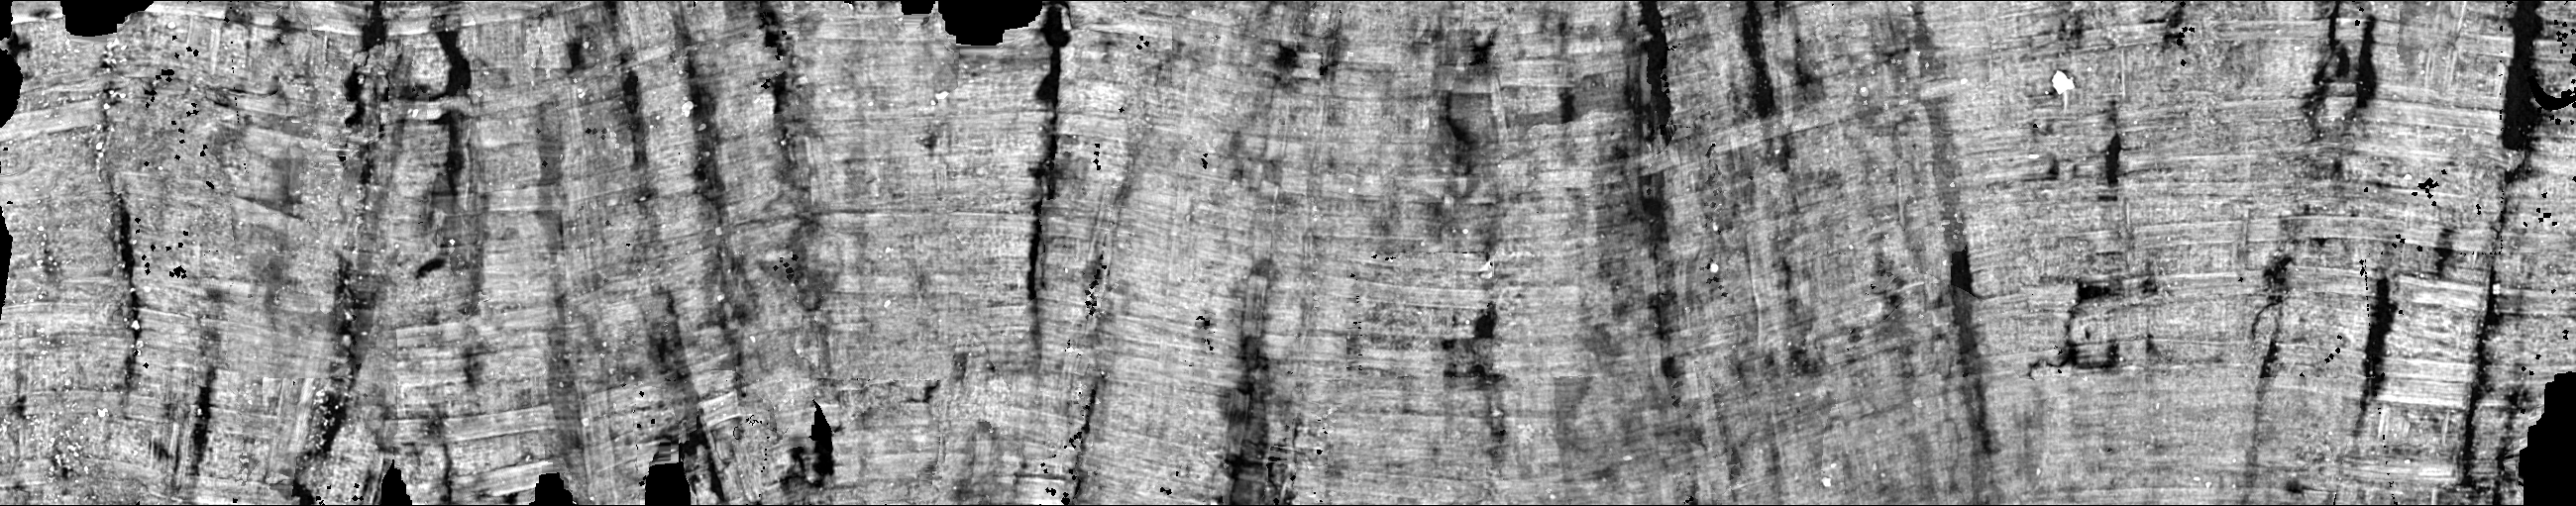
\includegraphics[width=\linewidth]{figures/unwrap_zoom.png}
  \caption{CT read-back from an accepted region of the developed $4\times5\times5$ experiment. The horizontal axis is developed arc length $u$ and the vertical axis is the scroll axis $v$. Continuous fibres and the perpendicular cross-hatch test the geometry and parameterization against the source volume; dark vertical bands are physical cracks and damage.}
  \Description{A wide grayscale developed CT texture with continuous fine fibre lines and several dark vertical crack bands.}
  \label{fig:unwrap}
\end{figure*}


\section{Repair in Parametric Space}
\label{sec:repair}

Flattening the sheet turns CT read-back into a repair instrument. Defects that are ambiguous on the folded surface become local evidence in the developed domain: a delaminated double layer covers the same $(u,v)$ twice; an off-sheet prediction is a dark island surrounded by papyrus texture; a bad atlas seam breaks a fibre that should continue. These operations are organized in the parametric domain, but they can update either 3D geometry (overlap selection and snap) or only UV coordinates (registration and relaxation). They complement the mesh-space repairs of Section~\ref{sec:cleanup}, which establish connectivity before image evidence is consulted.

\paragraph{Separating delaminated layers.} Where the papyrus has physically split into two nearly-coincident plies, the earlier geometric split cannot always tell them apart, and they arrive at the same $(u,v)$ and blur together in the read-back. Separating them is a two-energy problem. First we partition the multiply-covered region's triangles into layers with a lifted multicut~\cite{keuper2015efficient}: triangles adjacent in $(u,v)$ are joined by an {\em attractive} edge whose weight is their shared parametric edge length, while triangles that overlap at the same $(u,v)$ but lie far apart in 3D --- the delamination cue --- are joined by a strongly {\em repulsive} lifted edge. Minimizing the multicut objective
\begin{equation*}
  E_{\mathrm{cut}} = \!\!\sum_{(i,j)\,\mathrm{adj}}\!\! w_{ij}\,[\ell_i \neq \ell_j] \;+\!\! \sum_{(i,j)\,\mathrm{ovl}}\!\! |w_{ij}|\,[\ell_i = \ell_j]
\end{equation*}
over triangle labels $\ell$ (Kernighan--Lin, at least two clusters) keeps a connected ply together while forcing the two overlapping sheets onto different labels. Second, we decide which ply to keep with a {\em quilting energy}, the min-error boundary of image quilting~\cite{efros2001image}: we raster the CT intensity of each candidate ply and of the surrounding clean {\em anchor} sheet, and score the ply by the mean intensity discontinuity along their shared seam,
\begin{equation*}
  E_{\mathrm{quilt}} = \frac{1}{|\partial|}\sum_{p \in \partial} \bigl| (v^{L}_p - \bar v^{L}) - v^{A}_p \bigr|,
\end{equation*}
where $\partial$ are the seam-adjacent pixels and $\bar v^{L}$ removes any per-ply brightness offset. Because papyrus is near-uniform in mean brightness, $E_{\mathrm{quilt}}$ is dominated by whether the fibre pattern {\em lines up} across the seam; we keep the substantial ply that minimizes it --- the one whose texture best continues the surrounding sheet --- and relocate it to its own place in the atlas.

\paragraph{RAW-guided surface snap.} The U-Net occasionally places a surface patch in a dark inter-sheet gap rather than on papyrus (Fig.~\ref{fig:snap}, top). Snap is a current production stage, though its target objective is still being refined. A contrast-sensitive binary graph cut~\cite{boykov2001fast} first labels dark and supported vertices in the developed texture. For each dark island, samples are taken at signed depths along a stable across-sheet radial direction. A geometric occupancy query excludes the island's own neighbourhood and stops a ray before it enters any other mesh, so no candidate can cross an intervening wrap. An island without a supported boundary or an admissible free-space target remains an anchor and is not moved.

The first repair pass chooses target depths {\em jointly}, not as independent intensity maxima. Candidate positions for vertex $i$ are sampled at an odd number of signed depths $d_i$ along its across-sheet radial direction; the data cost $Q_i(d_i)=|v_{\mathrm{RAW}}(i,d_i)-\bar v_i|$ is the quilting mismatch between the RAW intensity sampled at that depth and the clean-boundary intensity $\bar v_i$ propagated inward from the island's nearest supported rim, so a candidate is cheap exactly when it {\em continues} the surrounding papyrus signal. A displacement penalty $\alpha|d_i|$ prefers small moves, and neighbouring labels pay a truncated-linear discontinuity cost,
\begin{equation*}
 E_{\mathrm{snap}}(d)=\sum_i \bigl(Q_i(d_i)+\alpha |d_i|\bigr)
 +\lambda\!\sum_{(i,j)\in E}\!\min\!\left(\tau,|d_i-d_j|\right),
\end{equation*}
which is optimized by alpha expansion (weights in Appendix~\ref{app:terms}). A zero-displacement label is always available, and a vertex with no legal target is forced to it, so unfixable vertices double as barriers that stop a target field from jumping to the far side of a sheet. The selected targets drive a screened-Laplacian displacement solve with clean vertices pinned. Solved vertices that violate occupancy are reverted. The purpose of the quilting term is coherence: a repaired island should continue the surrounding fibre pattern rather than chase whichever bright voxel happens to be nearest.

A second, global {\em recto refinement} addresses the fact that papyrus placement is not an intensity-maximum problem. Along the outward line it searches for an oriented dark-to-bright RAW transition, scores the transition with a local tangent-tensor quality estimate, and solves a smooth scalar displacement field over the mesh. Unsupported regions remain anchored; Jacobi updates, slope limits, damping, occupancy tests, and per-vertex reversion keep the pass conservative. This second objective is currently under real-data A/B evaluation. It improves the physical meaning of the target, but snap is not yet perfect in the crumpled core and is reported as such rather than omitted from the pipeline.

\begin{figure}[t]
  \centering
  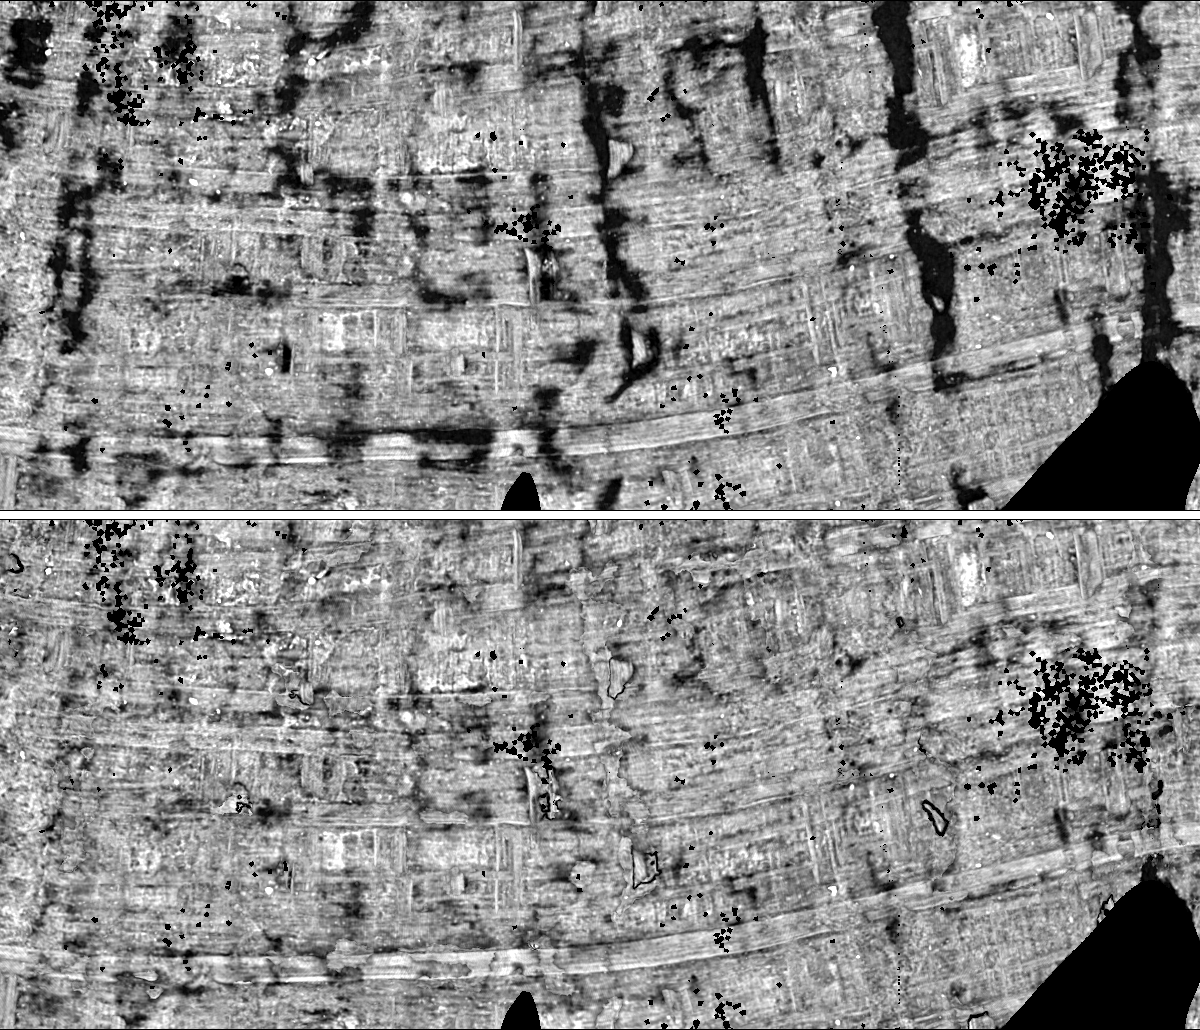
\includegraphics[width=\linewidth]{figures/snap_beforeafter.png}
  \caption{RAW-guided off-sheet repair, before (top) and after (bottom), on one developed region. Dark islands with supported boundaries are assigned coherent, occupancy-safe target depths and moved by a smooth solve. Persistent dark speckle is left in place when the evidence indicates real cracks or supplies no safe target.}
  \Description{Two grayscale CT texture crops. The lower repaired crop has more continuous bright papyrus texture while isolated dark cracks remain.}
  \label{fig:snap}
\end{figure}

\paragraph{Parameter-domain finalization.} After geometry repair, neighbouring ribbons are welded in UV and a quilting-based registration warp corrects residual $u$ offsets while preserving the established winding. The optional in-house relaxation combines symmetric Dirichlet distortion~\cite{smith2015bijective} with a fibre-alignment term derived from the structure tensor~\cite{bigun1987optimal}, and rejects any step that flips a triangle. It remains an experimental diagnostic: in the verified-patch test it worsened mean stretch and left flips, so the accepted local workflow delegates final flattening to Villa. For whole-scroll atlases, only registration candidates that improve seam mismatch and preserve coordinate validity are retained.

\paragraph{Collision-safe ribbon fitting.} The winding lift decides {\em which} wind each chart occupies; what remains is to turn the registered atlas into a single ribbon whose rows do not pass through one another. We slice the placed geometry at constant $v$ and sample each row at a common $u$ isovalue spacing, recording for every sample its position and unit tangent in the plane normal to the scroll axis. Samples that coincide in 3D within a local tolerance {\em and} agree in tangent are merged; those that coincide but disagree are recorded as conflicts rather than averaged, because a disagreeing tangent is the signature of two different wraps, not of noise. Each row is then fitted on a coarser control spacing by a least-squares problem combining observation position, a zero-curvature smoothness term, and a tangent term that integrates unit progress in $u$ (weights in Appendix~\ref{app:terms}). Where a row has no support, a bridge is admitted only if its chord is metrically plausible: a chord longer than $1.25\,\Delta u$ plus a small slack is rejected outright, on the principle that a metrically impossible bridge is evidence of a topology error and not a gap to be filled.

The fitted rows are then registered by smoothing each chart's $U$ shift along $v$, and finally audited for collision {\em exactly}. Rather than scoring occupancy on a grid, each round runs exact pairwise tests between rows and applies a fixed fraction of the computed escape, repeating until the ledger stops improving; an optional pass aligns the phase of adjacent rows against the RAW texture. This is the terminal stage of the whole-scroll path, and like the winding lift it reports its residual overlaps instead of declaring the surface verified.

Every fitted edge that is absent carries the gate that removed it. Measured on a default end-to-end run of the $4\times5\times5$ fixture --- stock parameters throughout, not the tuned winding campaign reported above --- the ribbon carries 9.1\% of the observed atlas area; the audit attributes the remainder to unbridgeable $u$ gaps (40.7\%), the vertical metric cut (26.9\%), topology cuts (19.4\%), and the horizontal metric cut (2.5\%), with rows outside the $v$ lattice, absent $u$ support, sub-grid islands, crossings, and geometry mismatch together accounting for the final 1.4\%. We report the breakdown rather than the single number because the reasons are actionable in a way the fraction is not: a $u$ gap is missing atlas, whereas a topology cut is the ribbon declining to bridge two wraps, and only the first is a coverage problem. A hole here is auditable evidence about the underlying atlas, not a silent omission.


\section{Interfaces and Downstream Integration}
\label{sec:integration}

\paragraph{Remote-volume workflow.} The public \texttt{scrollunwrap} entry point streams an OME-Zarr region from anonymous or authenticated S3 storage, sends the selected voxels to the in-memory C mesher, and can continue through preview and \texttt{tifxyz} output without first materializing a TIFF cube grid. It also supports local arrays, mesh-only operation, independent cube and flattener timeouts, and graceful cube skipping. All outputs carry the true $(x,y,z)$ origin and scale, so the resulting OBJ is immediately viewable and its atlas indexes the source volume rather than an internal cube convention.

\paragraph{Embeddable implementation.} One versioned public C header exposes cleanup, split, topology, reconstruction, remeshing, weld, and full volume-to-mesh operations. A consumer can use a static library, a shared library, or a runtime-loaded ABI table; cross-runtime allocation, structured status, progress, timeout, cancellation, and provenance are explicit. The CMake build is exercised as an embedded consumer and on Linux/GCC. MLS can run through the reference C path, OpenMP, an optional FP32 CUDA backend, or the research CubeCL CUDA backend, while every backend feeds the same geometry and topology gates. These interfaces make the workflow usable as a library rather than a chain of research executables.

\paragraph{Trust-aware application handoff.} A clean local component enters \texttt{villa-patch}: ScrollFiesta preserves its intermediate ribbon, quilting, and snap artifacts, Villa performs the authoritative final flatten, and the official loaders and overlap connector validate the result before it is registered as a verified patch. Larger uncertain surfaces enter VC3D through \texttt{ScrollFiesta: Generate Spiral Hints}. The command creates a new provenance-bearing \texttt{scroll-hint}/\texttt{unverified} segment, supports progress and cancellation, reloads the surface, and can add it to the active Spiral fit; it never overwrites its source. This separation allows useful whole-scroll feedback experiments without promoting an unresolved winding topology to verified papyrus.


\section{Current Results and Validation}
\label{sec:results}

We report topology and downstream validity separately because a visually clean mesh can be unusable if it contains even one phase-shortcut fusion.

\begin{figure*}[t]
  \centering
  \begin{subfigure}[b]{0.48\linewidth}
    \centering
    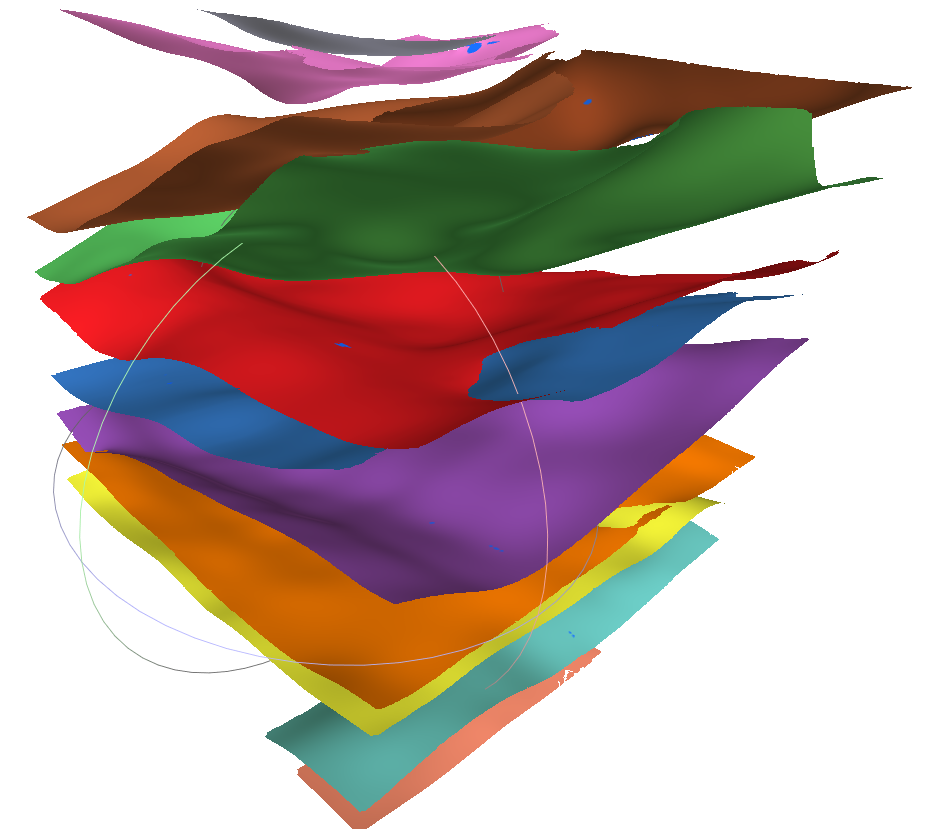
\includegraphics[width=\linewidth]{figures/kaggle_cube_118632705.png}
    \caption{Source cube 118632705 (11 sheets)}
    \label{fig:kaggle_a}
  \end{subfigure}
  \hfill
  \begin{subfigure}[b]{0.48\linewidth}
    \centering
    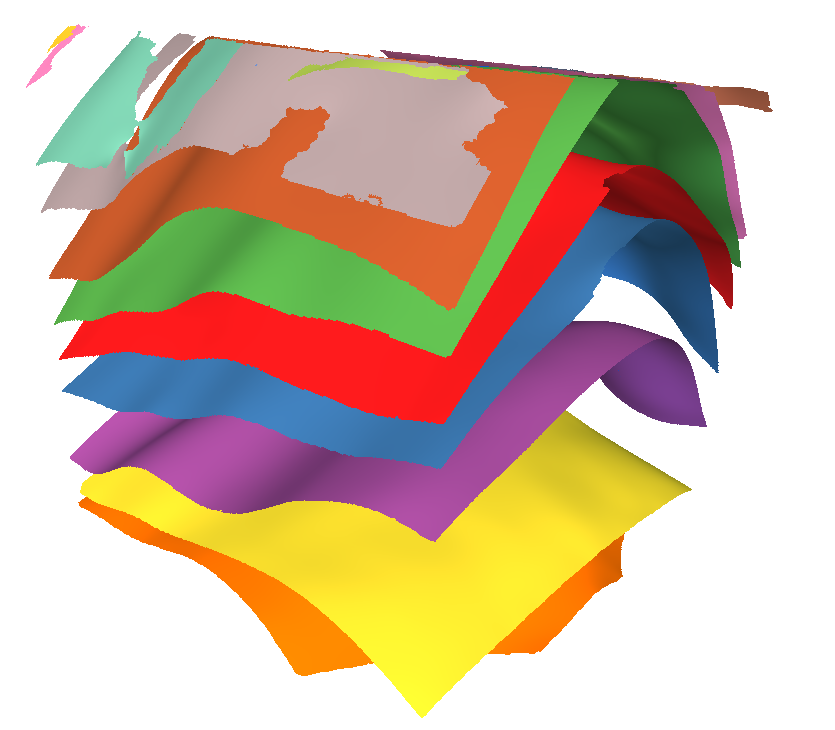
\includegraphics[width=\linewidth]{figures/kaggle_cube_3394433588.png}
    \caption{Source cube 3394433588 (15 sheets)}
    \label{fig:kaggle_b}
  \end{subfigure}
  \caption{Two dense Vesuvius Challenge training cubes after single-sided reconstruction and overlap separation. The roughly two-million-point inputs are divided into 11 and 15 component-coloured sheets before the current CVT/RVD level-of-detail stage.}
  \Description{Two coloured triangle-mesh stacks showing many separated, approximately parallel papyrus sheets in dense voxel cubes.}
  \label{fig:kaggle_cubes}
\end{figure*}

\begin{figure*}[t]
  \centering
  \begin{subfigure}[b]{0.360\linewidth}
    \centering
    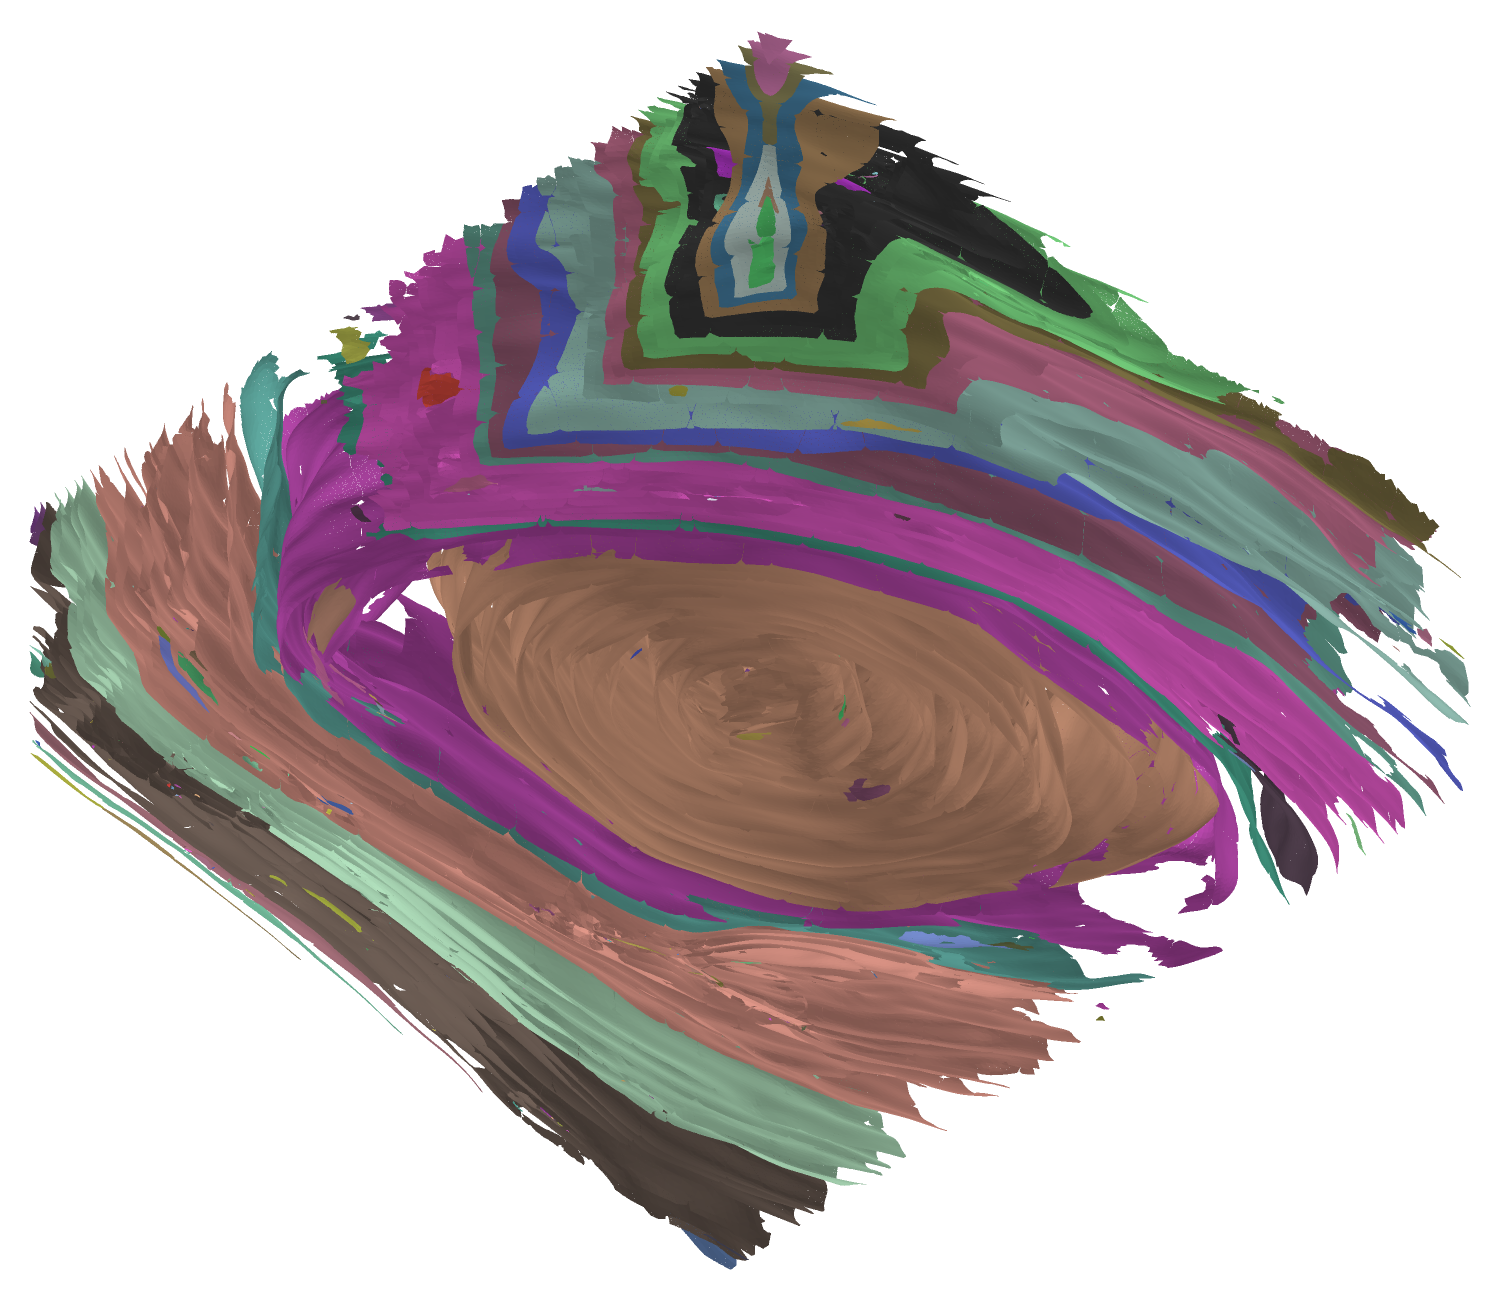
\includegraphics[width=\linewidth]{figures/mesh_10x10x10.png}
    \caption{PHerc0139, $10\times10\times10$ cubes: geometry}
    \label{fig:scale_10x_mesh}
  \end{subfigure}
  \hfill
  \begin{subfigure}[b]{0.620\linewidth}
    \centering
    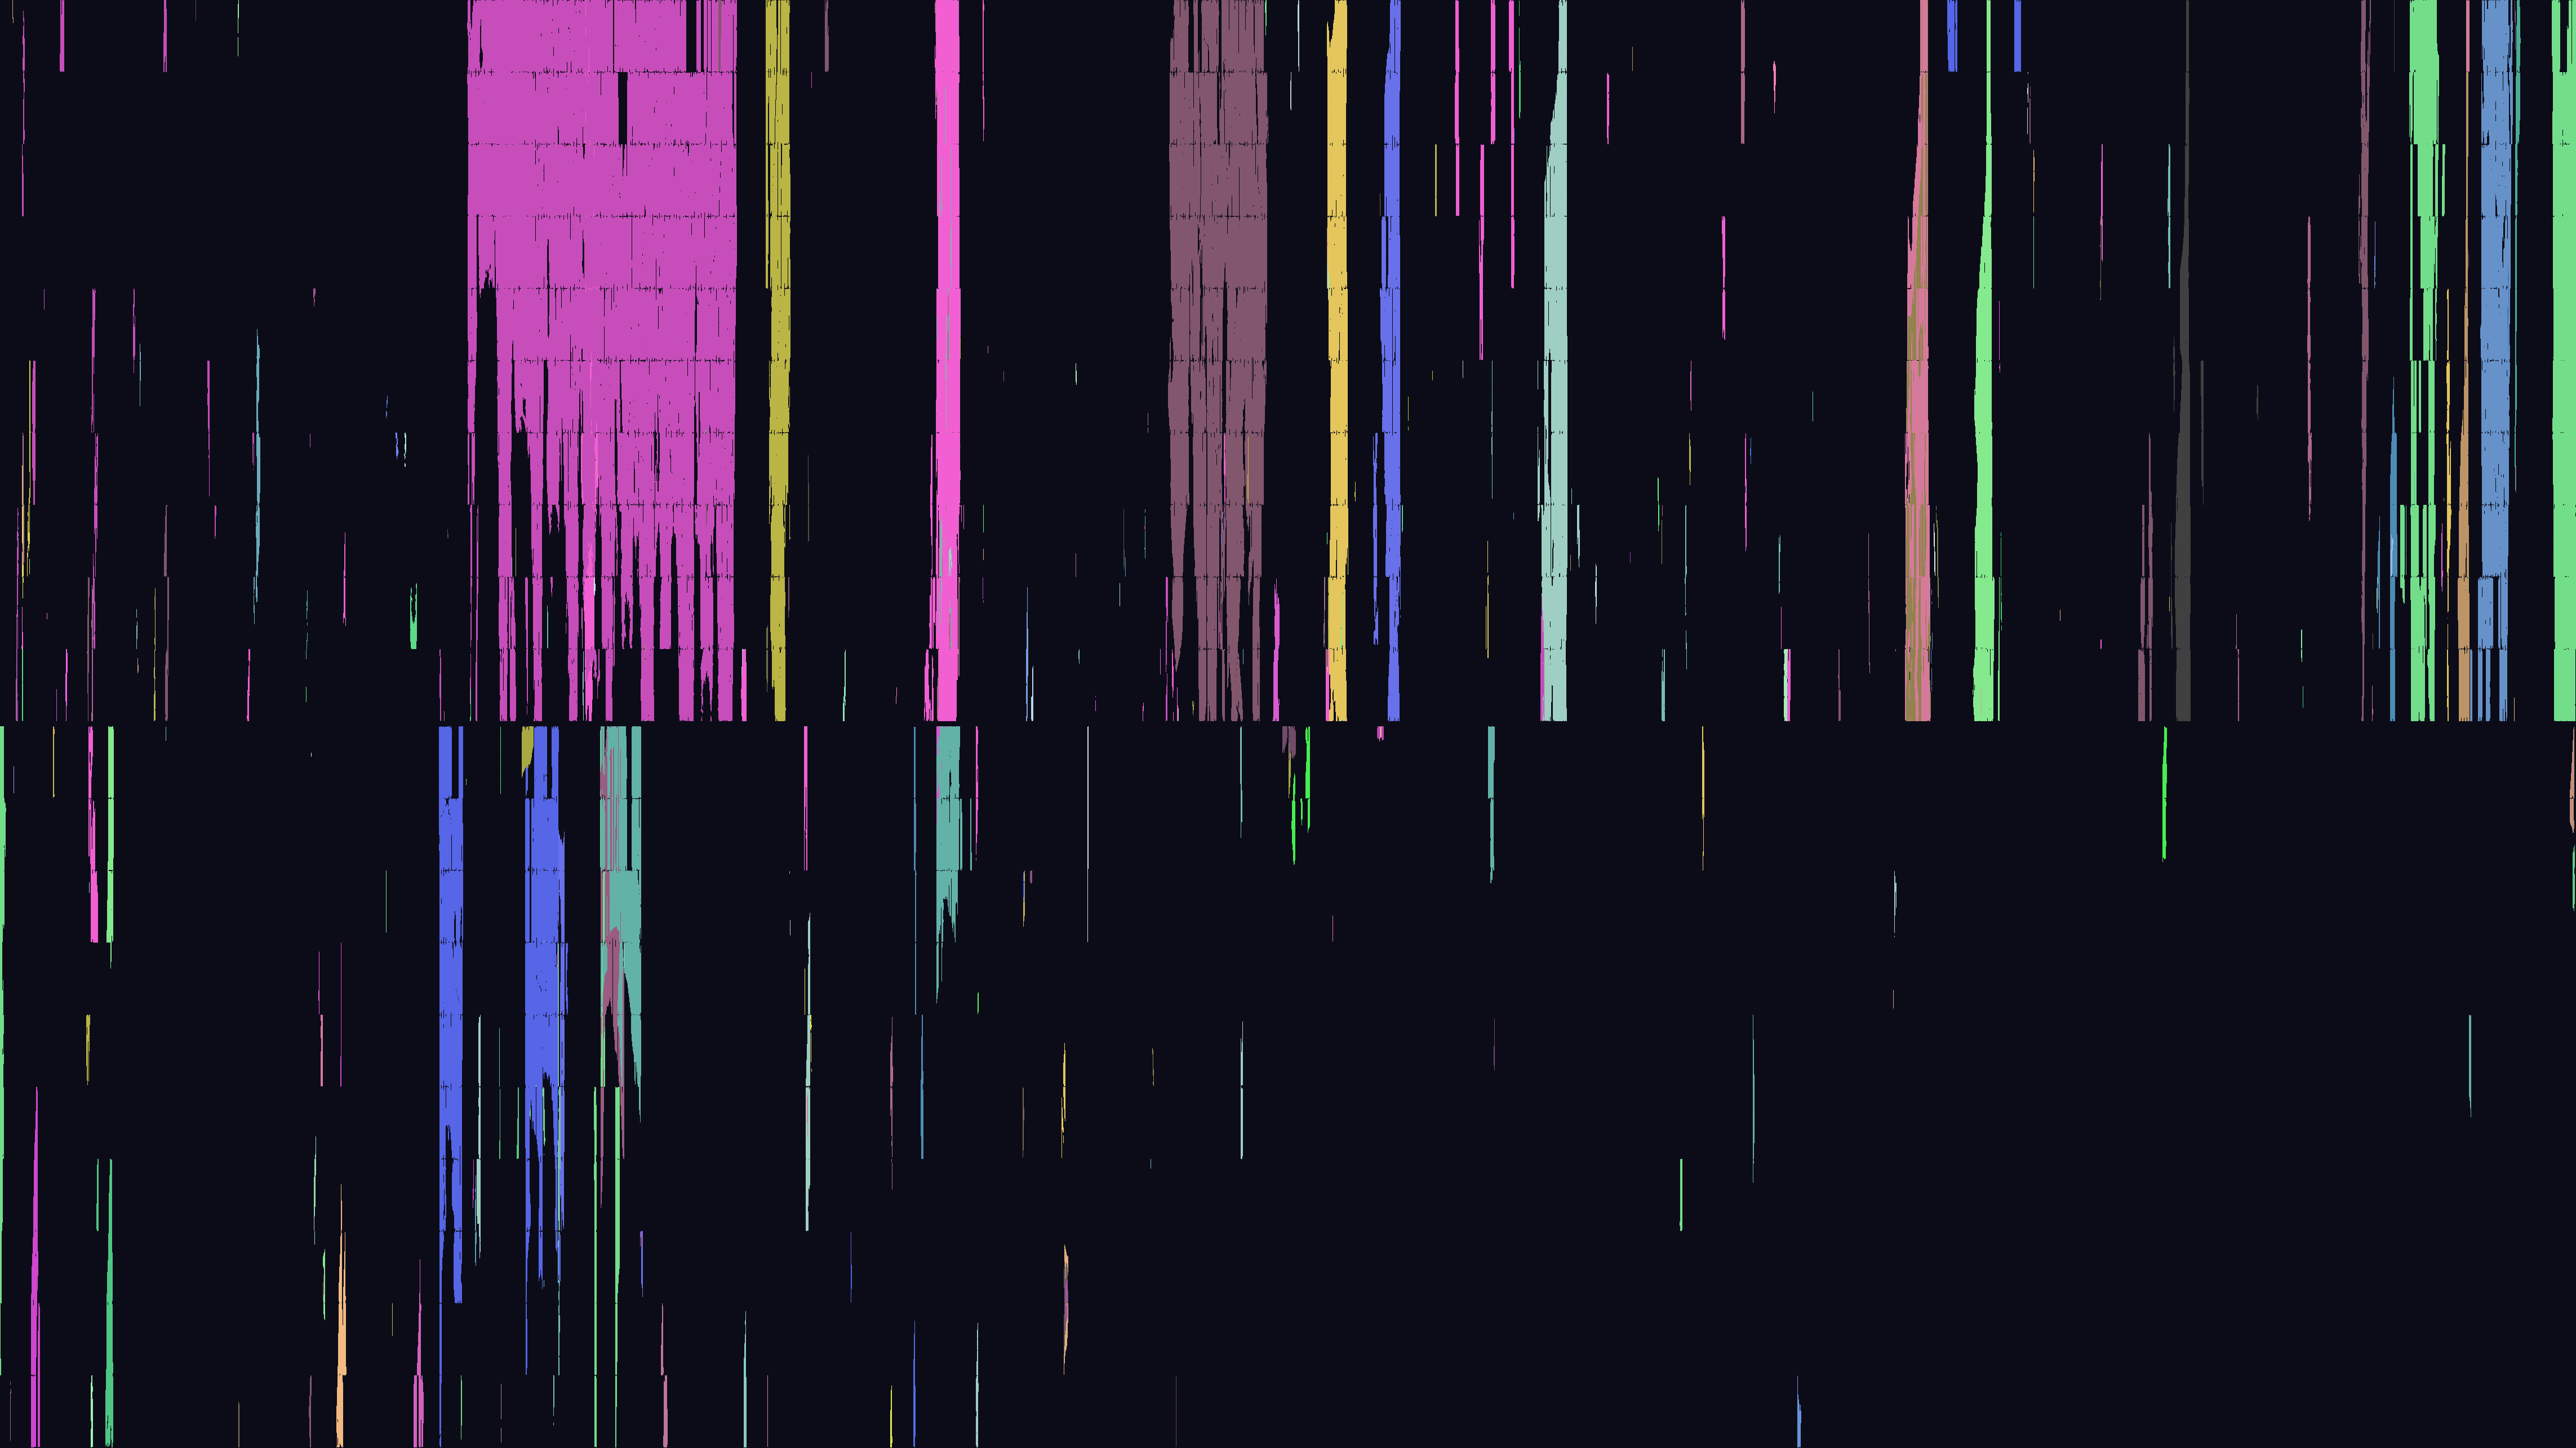
\includegraphics[width=\linewidth]{figures/atlas_10x10x10.png}
    \caption{PHerc0139, $10\times10\times10$ cubes: the registered atlas, cut into two rows}
    \label{fig:scale_10x}
  \end{subfigure}

  \medskip
  \begin{subfigure}[b]{0.735\linewidth}
    \centering
    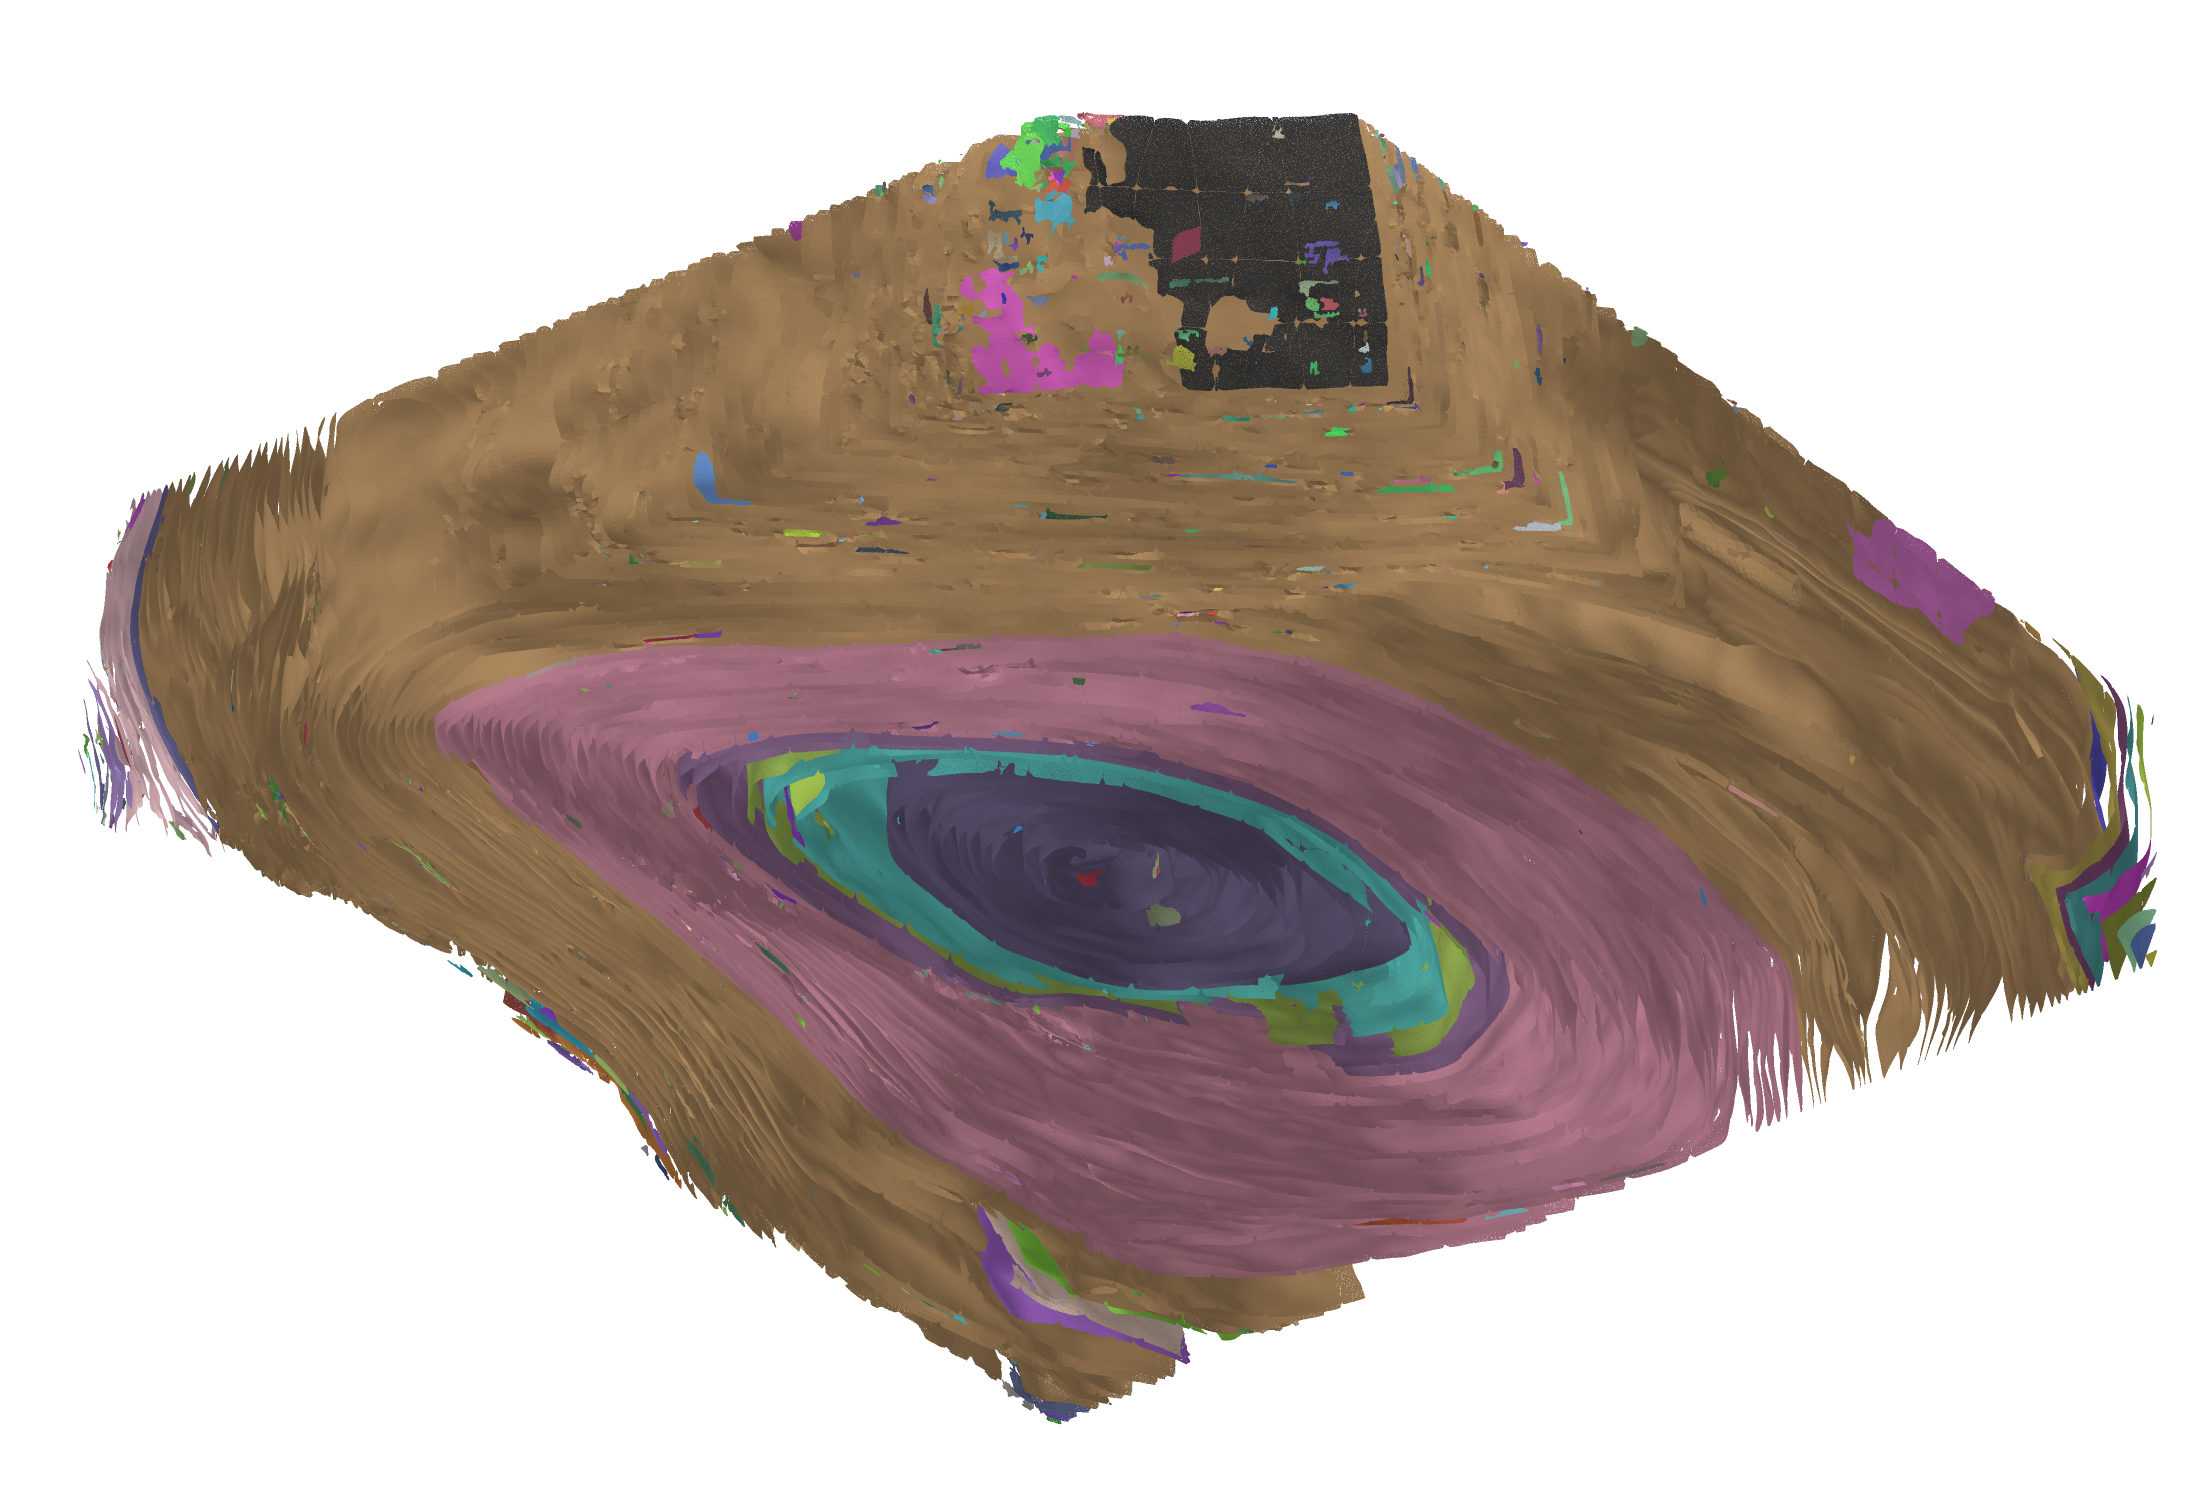
\includegraphics[width=\linewidth]{figures/mesh_4x21x21.png}
    \caption{PHerc0139, $4\times21\times21$ cubes: the band geometry (1,702 cubes)}
    \label{fig:scale_21x_mesh}
  \end{subfigure}
  \hfill
  \begin{subfigure}[b]{0.245\linewidth}
    \centering
    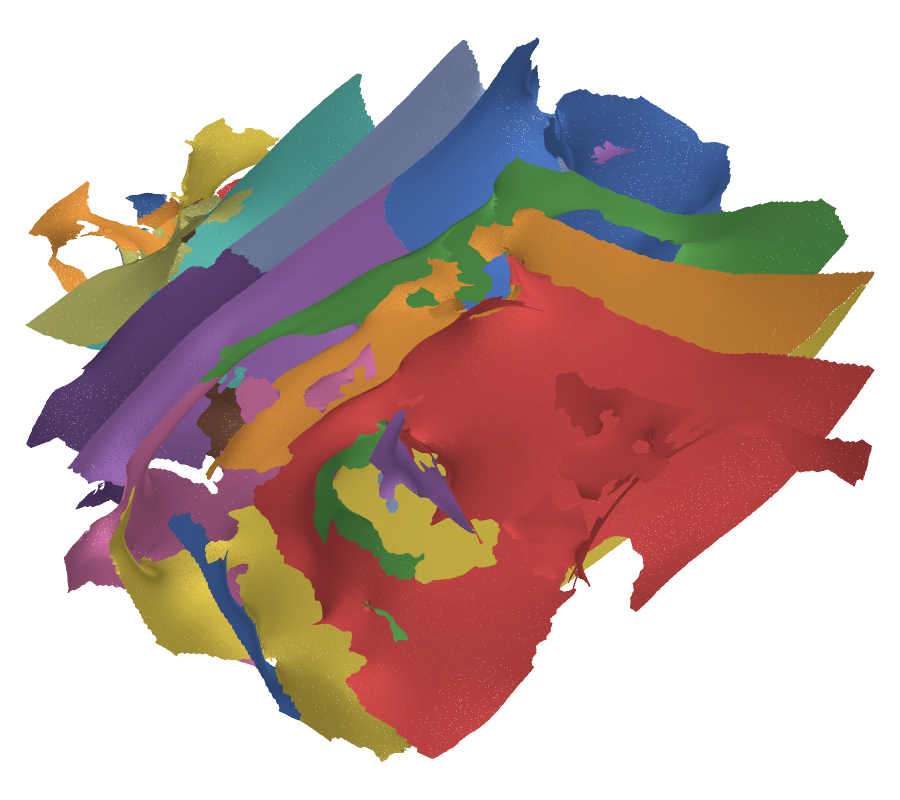
\includegraphics[width=\linewidth]{figures/pherc1203_cube.png}
    \caption{PHerc1203, one reconstructed cube}
    \label{fig:scale_1203}
  \end{subfigure}
  \caption{The same implementation beyond the $4\times5\times5$ fixture. (a) The thousand-cube PHerc0139 block in world space, cut at mid-height along the scroll axis to expose the recovered wraps spiralling around the umbilicus; colour identifies the welded atlas group, as in (b). (b) The same block carried through registration and the winding lift: the large welded groups survive as contiguous single-colour regions separated along $u$, which is the property the lift exists to produce, while the sparser second row is the volume's tail. (c) The full $4\times21\times21$ band --- 1,702 reconstructed cubes in world space, coloured by welded group, the geometry behind the stripwise atlas experiments. (d) A PHerc0139-trained configuration applied unchanged to a PHerc1203 cube, separated into component-coloured single-sided sheets. These runs demonstrate that the path scales and transfers; the winding and collision gates of Section~\ref{sec:repair} have not yet been run at these sizes.}
  \Description{Four panels: a cutaway render of a large spiral scroll block with wraps in distinct group colours, a wide two-row raster of a large unrolled atlas with contiguous coloured regions, a long slab-shaped render of many concentric papyrus wraps coloured by group, and a component-coloured render of separated sheets in a single reconstructed cube from a different scroll.}
  \label{fig:scale}
\end{figure*}

\paragraph{Per-cube extraction.}
Figure~\ref{fig:kaggle_cubes} shows two dense training cubes (source IDs 118632705 and 3394433588) with 2.07M and 1.92M raw points. Guarded BPA and the overlap separator recover 11 and 15 distinct single-sided sheets. Bridge separation and hole repair are shown in Fig.~\ref{fig:bridgesplit}. Across a difficult {\em PHerc1447} probe, however, adaptive BPA radii 1.20, 1.10, and 1.00 all retained nine broad fusions with maximum local span 18.70 turns while the boundary count increased. The quality gate therefore rejects radius reduction as a solution and requires those regions to be cut or quarantined.

\paragraph{Current 100-cube weld and CVT/RVD}
The latest complete central $4\times5\times5$ rebuild of {\em PHerc0139} processed all 100 cubes into a 264,268-face welded mesh (Fig.~\ref{fig:overview_mesh}), compared with 3.02M faces in the earlier collapse-only build. It has zero non-manifold edges and five same-direction edges. In the seam-band A/B, pinned CVT/RVD raised mean minimum triangle angle from $38.70^\circ$ to $43.38^\circ$, reduced triangles below $30^\circ$ from 24.88\% to 11.73\%, and changed 366,185 faces to 262,659 while preserving the audited boundary, component, Euler, and manifold counts exactly.

Those local topology counts do not certify scroll phase. The strict winding audit found 6,082 abrupt full-turn fusion edges; only 9.37\% lie near cube seams, which identifies prediction and per-cube reconstruction as the dominant source rather than welding. The experimental phase sever removed 9,650 faces (3.7\%), changed 28 connected components to 122, and reduced the abrupt-edge count to zero. Some resulting components still fail the broad local-span audit, so this output is exported only as an unverified hint. This negative result is important: manifoldness, orientation, and good triangles are necessary but not sufficient for a readable scroll.

\paragraph{Verified local flattening.}
On a clean 6,302-face {\em PHerc1447} component, the ScrollFiesta ribbon, quilting, and snap stages produced 21,218 valid cells, 20,873 valid quads, and no contested cells. The final output of Villa's maintained \texttt{flatboi} flattener contained 20,697 valid cells and 20,349 valid quads; the solve converged in five iterations, 87.1\% of the output grid rasterized, and the official loader, surface-index overlap connector, and full Spiral load-only path passed. By contrast, our optional relaxation left five flipped faces and changed mean stretch from 1.0298 to 1.0617, supporting the decision to delegate verified final flattening to Villa.

\paragraph{Geometric strip correction.}
The new audit found that 8,320 of 9,744 original plane-slice strokes traversed at least half a wrap internally, with a maximum span of 8.75 turns. Cutting 8,741 chains at 44,911 geometric wrap crossings produced 33,858 fragments; only 198 still span half a turn, and the maximum residual span is 0.68. The metric solve then changed developed advance per radial turn from 10.3\% to 103.1\% of a circumference. For comparison, posing the same monotone-constrained system as one large active-set QP hits a 235-second iteration cap without converging on the fragmented post-cut system, where the reduced LS--PAVA solve completes 11-round solves in 4.8--8.8 seconds. Direct-support transfer removed 2,304 of 172,116 candidate faces (1.34\%), including every one of the 696 zero-area UV faces that had survived neighbour filling. The corrected 169,812-face field has no degenerate UV triangle, no aspect ratio above 50, and no UV edge stretched more than $4\times$ its corresponding 3D edge. Rigid chart application preserves these local differences exactly.

\paragraph{Tabu winding repair.}
The locally metric field was still globally collapsed: 84.6\% of its within-group overlap pairs lay at least 0.75 pitch apart in radius, indicating different wraps at the same $u$. Table~\ref{tab:tabu} summarizes the discrete repair. The first per-chart search removed 95.4\% of exact overlaps but tore too many weld relations. Measuring the real field's wind ladder, adding same-wind lateral and happy-family terms, alternating with metric re-registration, and finally deriving graded bins from the weld chain reduced the exact count to 472 cross-group plus 1,402 within-group pairs, or 1,874 total (99.5\% below the registered field). A problematic 22-chart group's wrong-wind internal count fell from roughly 38,000 to 2, a second fell to zero, and the 324-chart group's count fell from 61,016 to 757. No happy-family bond tore; 41 usable weld relations remain torn and are the focus of the current stabilization work.

\begin{table}[t]
  \caption{Exact UV triangle-overlap progression on the $4\times5\times5$ atlas. ``Torn'' counts usable weld relations whose final integer-depth difference misses its target.}
  \label{tab:tabu}
  \centering
  \small
  \begin{tabular}{@{}lrrr@{}}
    \toprule
    Stage & Cross & Within group & Torn \\
    \midrule
    Registered field & 241,078 & 132,458 & 0 \\
    Per-chart tabu & 172 & 17,109 & 167 \\
    Alternating + graded & 535 & 3,447 & 38 \\
    Weld-chain bins & 472 & 1,402 & 41 \\
    \bottomrule
  \end{tabular}
\end{table}

The independent confirmation does not rely on the pair count alone. A four-round atlas bake produced a 47,514-by-511 CT strip with 30.4\% fill and 0.15\% multiple coverage; papyrus fabric remains continuous across chart seams. Per-winding OBJ layers show whether one colour moves coherently, while the $u$-radius plot separates formerly stacked winds. The exact-SAT stabilization work additionally records physical weld mismatch, because an integer target can look satisfied while the final seam is displaced by tens or hundreds of voxels; closing these stricter acceptance checks and establishing a verified global order of the separated group bands are the remaining steps.

An earlier $4\times21\times21$ band (Fig.~\ref{fig:scale_21x_mesh}) was parameterized as four axial strips using one winding calibration. Exact \texttt{tifxyz} welding retained 51,469,897 valid pixels across 166 wraps, with continuous fibres at strip boundaries, and arc registration reduced controlled seam texture mismatch by four to six times. That long band has not yet been rerun through the new global tabu stage. The $4\times5\times5$ VC3D demonstration carried a 544,178-cell unverified hint into Spiral feedback; a second correction reduced the active hint loss from 81.0648 to 13.0018 (83.96\%) and improved symmetric RMS by 10.31\%. These numbers measure the feedback channels; the underlying core surface is gated separately.

\paragraph{Snap and RAW-guided repair.}
Figure~\ref{fig:snap} demonstrates the present behaviour: supported dark islands move onto a coherent papyrus signal while anchorless cracks remain. The first-stage graph cut, occupancy barrier, joint quilting target, and screened solve are implemented in the pipeline; the oriented recto-transition pass is also implemented and undergoing real-volume comparison. The remaining failures concentrate in folded, delaminated core geometry, where candidate direction and ownership are ambiguous; the correction stays conservative there, and every vertex displacement is individually revertible.

\paragraph{Performance and backend parity.}
An OpenMP/MLS engine rewrite reduced one recorded $4\times5\times5$ mesh stage from 1,996\,s to 88.7\,s with byte-identical output, and removal of two hidden quadratic searches reduced the corresponding weld kernel from 351\,s to 79\,s, also byte-identically. The latest complete build meshed its 100 cubes in 129.2\,s and completed the full weld in approximately 9.3 minutes; pinned band CVT/RVD is now the dominant cost. On a captured 399,741-point {\em PHerc1447} cloud, five CubeCL CUDA MLS passes took a median 234.741\,ms and differed from the C reference by at most 0.000594 voxels. A complete-cube comparison took 73.654\,s versus 488.211\,s for the C path, approximately $6.6\times$ faster, while retaining the same downstream audits.


\section{Conclusions}
We present ScrollFiesta, a complete library for meshing and unwrapping of the Herculaneum papyri. It includes volume ingestion, single-sided reconstruction, topology repair, CVT/RVD level of detail, guarded cube welding, local or whole-scroll parameterization, CT-guided repair, collision-audited ribbon fitting, and verified or explicitly unverified handoff to Villa. Our central design choice is to preserve evidence and trust through the whole path. A manifold mesh is not assumed to be one sheet; a low collision count is not assumed to prove continuous seams; and an attractive CT raster is not assumed to establish global winding order.

\paragraph{Limitations and Future Work.}

The complete geometry weld has been validated on $4\times5\times5$ cubes; the $4\times21\times21$ result validates the earlier stripwise parameterization and atlas assembly, not a fully hierarchical geometry weld or the new global winding lift. We include preliminary results in the official repository. The local metric and global integer solves are now separate, but their interface is not yet certified. Direct-support gating trades 1.34\% of candidate faces for a non-degenerate local map. The best confirmed tabu run leaves 1,874 exact overlaps and 41 torn weld relations, and group bands that are locally separated are not yet globally ordered. The stabilization work is therefore moving exact triangle collision into the search, rejecting same-cube false weld evidence, and auditing physical seam displacement in addition to integer depth. Our ongoing agenda is to fit a ribbon to the observations created by the sheet, following the Strokestrip paradigm, but this remains ongoing work.

We note that the welded mesh also does retain core fusions concentrated away from cube seams, and the present RVD objective is not phase-aware. While our snap mechanism does use a principal quilted energy, it now needs controlled real-world data comparisons for both the joint target field and oriented recto transition, especially where delamination makes direction and ownership ambiguous. Pinned seam-band CVT/RVD remains the dominant weld cost, and this still remains prohibitively expensive for large cubes. Finally, we note that we now need to design better evaluations. At present we report retained area, manifoldness, local metric distortion, winding separation, exact collisions, seam displacement, fibre continuity and provenance together, but no single score yet captures the failures that make a scroll unreadable.


\appendix
\section{Developments Since the May 31 Update}
\label{app:developments}

This appendix lists the material changes implemented or validated between June 1 and July 30, 2026, relative to the May 31 progress report. The main paper describes the resulting current system; this list records the delta, with each new module described once, as it now stands. As of July 30 the whole-scroll atlas path is no longer split between a public repository and a private research tree: the winding lift, the registration solve, and the ribbon fit are all in the public repository, and the $4\times5\times5$ PHerc0139 chain from cube meshing through the fitted ribbon reproduces the research tree's results there. Publication is not verification --- the stabilization gates described above still govern what may be called verified papyrus --- but the evidence is now inspectable rather than described.

{\small
\begin{itemize}
  \setlength{\itemsep}{0pt}
  \item \textbf{Ingestion.} The public \texttt{scrollunwrap} workflow: authenticated or anonymous S3/OME-Zarr regions, local arrays, mesh-only operation, independent timeouts, graceful cube skipping, previews, and \texttt{tifxyz} export.

  \item \textbf{Embeddable API.} A one-header, versioned C ABI and CMake targets for static, shared, and runtime-loaded use, including true XYZ coordinates, explicit allocation, status and provenance, progress, cancellation, and the public \texttt{sf\_weld} operation, with direct, runtime-load, cancellation, and embedded-consumer tests.

  \item \textbf{Portable acceleration.} Clean Linux/GCC builds. MLS now runs through one projection interface with OpenMP, optional FP32 CUDA, and research CubeCL CUDA backends, all feeding the same geometry and topology gates.

  \item \textbf{Per-cube extraction hardening.} Every separated piece is reconstructed from its relevant original voxel points; solid-slab and empty-input predictions are rejected up front; BPA carries the full guard set of Section~\ref{sec:percube}, including the wall guard and the per-seed integrated winding phase that refuses gradual multi-turn growth and re-seeds the next wrap as a distinct component; pinches are split, holes closed manifold-safely, handles severed repeatedly; component culling scores each component against its parent input rather than the whole-cube total, so cubes containing many sheets keep their valid wraps; halo ownership and degenerate-cloud handling are explicit.

  \item \textbf{CVT/RVD level of detail.} The remesher is a restricted CVT with area and boundary seeding, normal-anisotropic relaxation, surface projection, and restricted-Delaunay output; repaired QEM remains only as an explicit or fail-closed fallback.

  \item \textbf{Seam-band welding.} Local refinement around cube planes for BPA, orientation- and winding-gated micro-welds and closers, post-weld recoarsening, and pinned-boundary CVT/RVD accepted only when pins, boundary edges, manifoldness, component count, and Euler characteristic are preserved.

  \item \textbf{Native metric parameterization.} The slice-domain solve of Section~\ref{sec:unwrap}: exact slice-stroke extraction, branch-cut-free geometric winding increments, cuts where strokes snake across wraps, trust-gated geometric anchors, and a reduced least-squares solve with PAVA monotonic projection, with short-edge parameter-jump audits, RAW read-back, and the consolidated \texttt{scroll\_ribbon --raw} path. Direct slice support is separated from neighbour-filled diagnostic values so fabricated plateaus cannot emit faces, and the global field is applied by robust support-to-chart registration --- one additive shift per raw chart --- preserving every local UV edge difference. This corrected the real-data developed advance from 10.3\% to 103.1\% of one circumference per turn without extension-induced flips or shear.

  \item \textbf{Whole-grid atlas assembly.} PieceSet placement and ownership, \texttt{scroll\_whole} and \texttt{scroll\_unroll}, whole-grid snap, UV welding and relaxation, stripwise shared-winding decomposition, exact \texttt{tifxyz} welding, provenance masks, atlas manifests, and quilting-constrained arc registration.

  \item \textbf{Discrete winding lift.} The alternating discrete--continuous stage of Section~\ref{sec:unwrap}, introduced as a whole: a deterministic per-chart tabu search over integer winding depths (departed-value tenure, aspiration, fixed-point energies, deterministic tie-breaking) with single-chart, welded-group, lateral-neighbourhood, and graded-rewind moves; wind bins integrated along weld and lateral chains so scroll-axis wander cancels; a measured field ladder for the per-wind $u$ step; happy-family protection and same-wind lateral coupling across holes; an exact-SAT-verified leaderboard that always retains the input assignment; same-cube rejection for proximity welds; physical post-move weld-displacement diagnostics; and the alternating loop in which tabu owns winding while \texttt{AtlasRegister} owns continuous metric placement. On the pinned $4\times5\times5$ atlas this reduced 373,536 exact overlap pairs to 1,874, confirmed by per-round winding-layer OBJs, $u$-radius diagnostics, chart/group/move CSVs, and a CT validation bake with 0.15\% multiple coverage. Its stricter acceptance gates remain active research and keep the 99.5\% overlap result from being treated as verified.

  \item \textbf{RAW-guided snap.} Graph-cut dark-region detection, occupancy-safe candidate search, joint quilting-guided depth labels solved by alpha expansion, and a smooth pinned displacement solve with per-vertex reversion, plus a second global recto refinement that targets an oriented dark-to-bright transition; the recto objective remains under real-data evaluation.

  \item \textbf{Villa, VC3D, and Spiral.} The verified local-patch handoff through Villa's maintained flattener and official loaders, plus a non-destructive VC3D command that creates cancellable unverified Spiral hints with explicit provenance and can feed them into an active fit.

  \item \textbf{Topology and adaptive-extraction audits.} Abrupt-edge and broad branch-local winding tests, coverage and boundary gates, adaptive BPA radius trials, phase cutting, machine-readable reports, and the policy that unresolved broad fusions are quarantined rather than accepted because they look clean.

  \item \textbf{Seam-consistent whole-scroll registration.} Registration now has a single path: the exact max-confidence forest, scalar consistency polish, then the continuous \texttt{ArcReg} $u$-warp. On $4\times5\times5$ this took whole-turn seam error from 90.73\% to 1.67\% of pairs and $|\Delta u| < 2$ join completeness from 8.52\% to 82.91\%. \texttt{--audit} exits nonzero when turn-off exceeds 5\% or close-join completeness falls below 50\%, so file existence can no longer certify a fragmented result.

  \item \textbf{Winding topology across sparse grids.} Winding relations are preserved where the cube grid is sparse and neighbours are absent, so a missing cube no longer silently breaks the chain the registration and lift depend on.

  \item \textbf{Collision-safe ribbon fitting.} The terminal whole-scroll stage described in Section~\ref{sec:repair}: constant-$v$ slicing, tangent-aware duplicate merging, per-row least-squares fitting under position, curvature, and unit-$u$ tangent terms, metric rejection of impossible bridges, chart-shift registration, and an exact rather than grid-approximate collision audit, with per-edge rejection provenance. \texttt{atlas\_overlap\_fix} hands the ribbon a checkpointed atlas solution, making the two stages separately runnable and separately auditable.

  \item \textbf{Performance, memory, and robustness.} A rewritten OpenMP MLS engine and weld kernel with byte-identical output (Section~9), removal of hidden quadratic searches, \texttt{size\_t} arena sizes, bounded handle-sever scratch, KD-tree and QEM correctness fixes, and expanded component-coloured dumps, previews, CI, and unit coverage across the pipeline.
\end{itemize}
}


\section{Term Definitions, Default Constants, and the Tabu Procedure}
\label{app:terms}

This appendix defines every energy term the paper optimizes and records the default constants the public implementation ships with, so each stage is reproducible from the text. Lengths are in voxels and angles in turns unless stated; ``clearance'' refers to the measured $\sim$7-voxel minimum inter-wrap spacing of PHerc0139, the single geometric quantity from which most safety caps are derived.

\subsection{Per-Cube Extraction}
\label{app:extraction}

\paragraph{MLS projection} Each point $v$ takes the neighbours of its point cloud within a Wendland-kernel radius of 12 (approximately twice the local sheet thickness, so the far face of a thick prediction still carries weight and collapses), estimates a normal $n$ and weighted centroid $c$ from them, and moves only along the normal, $v' = v - ((v-c)\cdot n)\,n$. Restricting motion to the through-thickness direction is what prevents the in-plane contraction of centroid replacement at high iteration counts. Five iterations are used at extraction and twenty when a separated piece is re-projected from its parent's original points; points within 0.25 of one another are then welded, and a point with fewer than four neighbours is left in place. Determinism across cubes requires only that the read halo exceed the kernel radius by one voxel (13), so every owned point sees its full two-sided support.

\paragraph{Ball pivoting and guards} The pivot radius is $\rho = 1.2$, about $1.55\times$ the $\sim$0.77 projected point spacing: below ${\sim}1.1\times$ spacing, sparse sheets fall through the ball; above ${\sim}2\times$, the empty-ball test crowds with cocircular intruders. Triangle quality is insensitive to $\rho$ in this band (it is fixed by the point arrangement), so $\rho$ acts purely as a coverage/anti-merge knob. The wall guard rejects a candidate whose face normal is tilted more than ${\sim}70^\circ$ from the mean vertex normal ($|\cos| < 0.34$) {\em and} whose spanning edge exceeds 2.0 --- the conjunction fires on through-thickness fusion bridges and spares short-edged folds and rims. The per-seed growth gate integrates the branch-cut-free winding phase $w = r/p - \theta/2\pi$ along the advancing front and refuses a pivot once the accumulated phase leaves its tolerance band; the surface beyond is re-seeded as a new component. Non-separating handle loops shorter than 60 are severed after hole filling; a per-cube sheet has no legitimate scroll-scale handle, and the length bound is the safety margin.

\subsection{CVT/RVD Remeshing}
\label{app:cvt}

The remesher minimizes the CWF objective~\cite{xu2024cwf}, a centroidal Voronoi energy plus a normal-anisotropy term,
$E = \lambda_{\mathrm{CVT}} \sum_i \int_{\Omega_i} \lVert x - x_i\rVert^2 \, dA + \lambda_{\mathrm{NA}} E_{\mathrm{NA}},$
where $\Omega_i$ is site $i$'s restricted Voronoi cell on the surface and $E_{\mathrm{NA}}$ penalizes cell mass displaced off the local tangent plane, pulling samples onto creases. Each iteration solves, per site with fixed cells, the $3\times3$ system $(\lambda_{\mathrm{NA}} N_i + \lambda_{\mathrm{CVT}} m_i I)\,x_i = \lambda_{\mathrm{NA}} b_i + \lambda_{\mathrm{CVT}} m_i c_i$ ($m_i$, $c_i$ the cell's mass and centroid; $N_i$, $b_i$ the anisotropy normal equations), then projects $x_i$ back to the source surface. Both weights start at 1 and $\lambda_{\mathrm{CVT}}$ decays by 0.95 per iteration to a floor of $10^{-3}$; the pipeline runs 12 iterations, at which the decayed energy has converged. Uniform density places $0.0025\times$ the input face count in sites (minimum 50). At weld time the seam band is refined to 3.5-voxel triangles --- pinned by bridge priming, since a hinge ball reconstructs only when the front triangle's circumradius is below the bridge radius --- and recoarsened afterwards by guarded collapse of band edges shorter than 5, a cap deliberately below the 7-voxel clearance so no collapse can fuse wraps. The pinned-boundary variant makes every patch boundary vertex an immutable site (bit-exact, so the patch stitches back conformally), seeds the interior at the target spacing while keeping $0.85\times$ the local boundary segment length clear of the rim, and accepts a patch only if every pin is referenced, every consecutive boundary pair is still an edge, and manifoldness, component count, and Euler characteristic are unchanged; rejection is per $\sim$cube-scale tile, so one core fold cannot reject a whole seam.

\subsection{Slice-Stroke Metric Solve}
\label{app:slice}

The unknowns are one developed coordinate $u$ per slice sample plus one latent intercept per cross-section. Three row types feed the least-squares system: {\em arc-length rows} asking consecutive samples of a stroke to advance by their measured 3D arc length; {\em cross-section rows} tying each member sample to its cross-section's latent isovalue, weighted by a membership likelihood; and {\em continuation rows} joining two stroke endpoints on one slice with target $u_a - u_b = \tau \cdot (p_a - p_b)$, the tangent-projected physical gap, emitted only for mutually selected, sub-half-wrap joins. The geometric gauge $\varphi_{\mathrm{geo}}$ of Section~\ref{sec:unwrap} anchors only strokes whose geometric coordinate agrees with their measured arc length; the reduced system solves anchors-only with a small Tikhonov term on near-null directions. Five reweighting rounds (plus two at tightened $\sigma/3$) downweight outlier rows, and pool-adjacent-violators projection restores per-stroke monotonicity after each round, which is what makes the post-cut, fragmented system well-behaved where the earlier active-set QP was not.

\subsection{The Discrete Winding Lift}
\label{app:tabu}

\paragraph{Structures} A {\em chart} is one connected component of the retained mesh; since charts never share vertices across cubes, a chart is one cube's sheet. Two charts are {\em authentic neighbours} when at least 3 vertex pairs lie within 6 (twice the maximum bridge radius, deliberately below the 7-voxel clearance so a ``neighbour'' can never be the next wrap in) with contact normals agreeing to $|\!\cos| \ge 0.7$; a {\em welded group} is a connected component of that graph, i.e.\ one physically welded fragment. Before the search, faces whose UV/XYZ edge stretch exceeds $8\times$ are killed, and a per-chart wind reconciliation integrates weld gauge evidence over a maximum-confidence spanning forest, using only weld edges whose turn residual is below 0.25 and capping corrections at $\pm8$ turns.

\paragraph{Energy} $E(k)$ is as given in Section~\ref{sec:unwrap} with defaults $\lambda_o = 1$ per exact overlapping face pair, $\lambda_n = 4$ per contact-weighted torn turn, and $\lambda_r = 2$ per turn of Huber radial deviation. Weld edges weight $w_{ab}$ by physical contact count; lateral same-wind edges (same radius within 0.6 pitch, adjacent cubes, side by side within $\Delta u \le 200$) carry 8 contact-equivalents and target $t_{ab} = 0$; edges inside a happy family are boosted $8\times$. A steering-only variant downweights edges to a currently-colliding neighbour by $0.25$ when {\em ranking} candidate moves, but the canonical (unsteered) energy owns acceptance, best-tracking, aspiration, and stopping. The one-wind ladder --- the signed $\Delta u$ of moving one wind outward --- is the median over radially adjacent same-$u$ chart pairs; if too few pairs support it, the solver falls back to the calibrated spiral map. Exact overlap counting memoizes face-pair tests behind chart- and face-level AABB/sweep rejection, with cube provenance excluding pairs emitted by one cube.

\paragraph{Search} Depths span $k \in [-4, 4]$. Each iteration evaluates single-chart moves and the compound moves (whole welded group, lateral neighbourhood, graded rewind with bins from integrated radial climb, and compound relative-gauge regions), all in fixed-point $1/1024$ energy units so no platform's floating-point summation can reorder decisions. The best non-tabu move is applied --- or a tabu move, if it would beat the best energy ever seen (aspiration) --- and each departed depth is banned for 40 iterations. Ties break by fixed chart order. The search stops after 300 iterations without improving the canonical best, with a hard cap of 2{,}000. Every accepted state is archived; a leaderboard of candidates, always including the input assignment as state~0, is re-scored by exact SAT triangle intersection, and the winner is chosen on the exact count with the summed $|k|$ as tie-break. Physical weld displacement ($|\Delta u|$ at the contact, with counts of jumps above 25 and 100) is recorded per candidate, because an integer-satisfied target can still hide a large metric discontinuity.

\paragraph{Relayout} With the winning depths frozen, a continuous per-chart $u$ re-registration restores metric seam agreement: intact weld edges become closure springs, same-depth laterals keep-together springs, and radially adjacent pairs enforce at least the measured per-wind separation so the continuous stage cannot re-collapse what the search separated. Charts are weighted by face count (clipped at $0.25\times$ the mean), deviation across any intact topology edge is budgeted at 25, and the re-layout is accepted only if an independent exact-overlap recount does not worsen; otherwise it is reverted and the pure tabu placement stands.

\subsection{Quilting and Snap Terms}
\label{app:snap}

In $E_{\mathrm{snap}}$, candidates for a dark vertex are sampled at 33 signed depths over $\pm8$ along the across-sheet radial direction, marching in 0.25 steps and stopping at occupancy 0.9 against foreign geometry. The data term weights are $30$ on the quilting mismatch $|v_{\mathrm{RAW}} - \bar v|$ and $200$ on the normalized displacement; the truncated-linear smoothness uses $\lambda = 2000$ with $\tau = 4$, optimized by alpha expansion. The dark-region detector is a binary graph cut with intensity threshold 64, contrast-sensitive weight $\lambda_{\mathrm{cut}} = 20$, and $\sigma = 30$, tuned inclusive (false positives are recoverable; a missed dark island is not). The screened-Laplacian move pins clean vertices at weight $10^4$, pulls island vertices toward their targets at $\alpha/(1-\alpha)$ per adjacent edge with $\alpha = 0.85$, caps displacement at 8, and reverts any vertex whose solved position violates occupancy.

\subsection{Collision-Safe Ribbon Fit}
\label{app:ribbon}

Rows are sliced every 4 in $v$ and sampled every 2 in $u$; duplicates merge when samples coincide within the local tolerance {\em and} tangents agree to $\cos \ge 0.5$, and conflicting-tangent coincidences are recorded, not averaged. Each row is fitted on a 16-voxel control spacing minimizing
$\lambda_p \sum \lVert P(u_i) - o_i \rVert^2 + \lambda_s \sum \lVert P'' \rVert^2 + \lambda_t \sum \lVert P' - \hat t \rVert^2$
with $(\lambda_p, \lambda_s, \lambda_t) = (1, 8, 4)$, where the tangent term integrates unit metric progress in $u$. Unsupported gaps are bridged only up to 512 and only if the chord passes the $1.25\,\Delta u + 4$ stretch test. Chart $U$ shifts are then smoothed along $v$ (weight 16, six bidirectional sweeps), and the exact collision audit repeatedly applies $0.35$ of each computed escape for up to eight rounds, stopping when the ledger stops improving.


\bibliographystyle{ACM-Reference-Format}
\bibliography{bibliography}

\end{document}
\endinput
%%
%% End of file `sample-acmtog.tex'.
